%--------------------
% document principal
%--------------------
% cal compilar amb `pdflatex -shell-escape main.tex`
% makeglossaries main
%--------------------
\documentclass[paper=a4,fontsize=11pt,twoside,parskip=half,BCOR12mm]{scrbook}
%%%%BCOR12mm  factor de correcció per enquadernació
%\usepackage[T1]{fontenc}
%------------- capçalera ----------------------
\input{capçalera.default}
\bibliography{bibliografia}
\ExecuteBibliographyOptions{annotation=true,backref=true,}
%\graphicspath{{imatges/}} %{{imatges/}{imatges/model/}}
%---------- Mode esborrany --------------------
%\includeonly{model-dades}
\usepackage[catalan]{todonotes} %%ús: \todo{text} \missingfigure{text}
\usepackage{fancyhdr}\pagestyle{fancyplain}\chead{\fancyplain{--- esborrany \today\ ---}{\footnotesize\today}}
%%\renewcommand{\headrulewidth}{0pt}
%----------------------------------------------
%\usetikzlibrary{shapes,arrows,positioning}
%\usetikzlibrary{calc}
%------------- format -------------------------
%%ús coma decimal sense espais:  2{,}5
\newtheorem{definition}{Definició}
\def\figureautorefname{figura} %ús: \autoref{}
\numberwithin{equation}{chapter}
\DeclareMathOperator*{\seg}{seg}
\DeclareMathOperator*{\ant}{ant}

\usepackage{longtable}

%glossaris
\usepackage[
          acronym,
          %nonumberlist,
          %toc,
          section,
          numberedsection=autolabel,
          sanitize=none, %pels accents en el vegeu
          ]{glossaries}
%\renewcommand*{\glspostdescription}{}%anul·la el punt final
\renewcommand*{\acronymname}{Sigles}%{Índex de sigles}??si té refs pàgines 
%Índex d'abreviacions?? si conté abreviatures o símbols
% \short<type>name,
\newglossary{notation}{not}{ntn}{Notació}
\newglossarystyle{estil-notation}{%
  \renewcommand{\glsgroupskip}{}% make nothing happen between groups
  \renewenvironment{theglossary}
  {\begin{longtable}{lll}
      % \caption{Notació dels SGSTM \label{tab:sgstm-simbols}}
      % \endfirsthead
      % \caption[]{Notació dels SGSTM (continuació)}
      % \endhead
          % \endfoot
          % \endlastfoot
    }{\end{longtable}}
  \renewcommand*{\glossarysubentryfield}[6]{%
    %\glstarget{##2}{##3}% the entry name
    \glstarget{##2}{\Glsentryname{##2}}% the entry name
    &
     %\space (##5)% the symbol in brackets
    \space ##4% the description
    &
    \space [##6]% the number list in square brackets
    \\
  }%
  \renewcommand*{\glossaryentryfield}[5]{%
    \\\pagebreak[3]\hline
    \glossarysubentryfield{##2}{##1}{##2}{##3}{##4}{##5}
    \hline
  }
}


\renewcommand{\seename}{vegeu}
\renewcommand{\entryname}{Notació}
\renewcommand{\descriptionname}{Descripció}

\makeglossaries


%\renewcommand{\glossarypreamble}{Text com a préambul}



%TERMES


%temps real
\newglossaryentry{TempsReal}{name={temps real}, description={(\emph{real time}), sistemes que han de respondre amb un temps determinat. A vegades també s'utilitza el terme com a adjectiu per a designar sincronització real amb el rellotge o per a indicar que l'usuari no percep retards. Allà on pugui causar confusió, utilitzarem sincronitzat o en línia (\emph{online}) per al segon significat.}
}





\newglossaryentry{SistemaGestioBaseDades}{name={sistema de gesti{ó} de base de dades}, description={(\emph{Data Base Management System})} }




%terme:SGBDR

\newglossaryentry{terme:SGBDR}{name={sistema de gestió de base de dades relacional}, description={(\emph{Relational Data Base Management System}). 
També anomenat 'object/relational' DBMS \parencite{date06}.
Totes les definicions són coherents amb \textcite{date:introduction} } }



%model, implementació
%Els SGBD es basen en teories matemàtiques que reben el nom de model de dades, un SGBD és una implementació d'un model de dades.
%Segons \citeauthor{date:introduction}, ``un model de dades és una definició abstracta, auto continguda i lògica dels objectes, de les operacions i  de la resta que conjuntament constitueixen la màquina abstracta amb la que els usuaris interactuen. Els objectes permeten modelar l'estructura de les dades. Les operacions permeten modelar el comportament''. Ara bé, \citeauthor{date:introduction} avisa que el concepte model de dades també s'usa per a definir una estructura persistent de dades concreta i per tant cal distingir adequadament la confusió entre els dos conceptes.
% Tal com fa Date, parlarem de model de dades en el primer sentit de màquina abstracta i a vegades ho abreviarem com a model.


%tipus,valor,variable,operador

\newglossaryentry{terme:SGBDR:domini}{see={terme:SGBDR},name={domini}, description = {(\emph{domain}), equivalent a tipus de dades.
Conjunt de valors. Cada domini té associat un conjunt d'operadors, en alguns casos fins i tot s'entén que el domini inclou els operadors (concepte de classe a orientació a objecte). Els tipus tenen una representació (estructura) o més d'una, és a dir els seus valors poden estar denotats per més d'un literal} }
\newglossaryentry{terme:SGBDR:tipus}{see={terme:SGBDR:domini}, name={tipus de dades}, description = {(\emph{data type}), a vegades solament 'tipus' (\emph{type}) o bé 'tipus de dades abstracte' (\emph{abstract data type}). Segons \textcite{date:introduction} en el context de model tots els tipus de dades han de ser abstractes} }

\newglossaryentry{terme:SGBDR:escalar}{parent={terme:SGBDR:domini}, name={escalar}, description = {Un tipus és escalar (\emph{scalar}) quan no té components visibles a l'usuari i és no escalar (\emph{nonscalar}) en cas contrari; no obstant, tant els escalars com els no escalars tenen representació, la qual pot contenir components} }


\newglossaryentry{terme:SGBDR:valor}{see={terme:SGBDR},name={valor}, description = {(\emph{value}), equivalent a objecte i instància.
'Constant individual' que és d'un tipus de dades. A vegades s'utilitza 'constant' per designar una  variable que mai canvia de valor, però aquest no és el cas d'aquesta definició} }
\newglossaryentry{terme:SGBDR:objecte}{see={terme:SGBDR:valor}, name={objecte}, description = {(\emph{object})} }
\newglossaryentry{terme:SGBDR:instancia}{see={terme:SGBDR:valor}, name={instància}, description = {(\emph{instance})} }

\newglossaryentry{terme:SGBDR:literal}{see={terme:SGBDR},name={literal}, description = {(\emph{literal}).
Símbol que denota un valor. Un valor pot estar denotat per més d'un literal. Segons aquesta definició literal no és equivalent a valor} }


\newglossaryentry{terme:SGBDR:variable}{see={terme:SGBDR},name={variable}, description = {(\emph{variable}).
Contenidor d'una aparició d'un valor. El valor que conté la variable pot ser canviat mitjançant l'operador d'assignació. En canvi els valors, per si mateixos, no poden ser actualitzats} } %A l'esquerra de l'operador d'assignació sempre hi ha variables, tot i que s'admeten simplificacions mitjançant expressions que són pseudovariables (p.ex. s[1] := 3 és equivalent a s := [s[0],3,s[2],..]).
%Les variables tenen adreces (\emph{addresses}) i per tant es pot apuntar (\emph{point to}) a les variables mitjançant els operadors de referència (\emph{referencing}), el qual retorna l'adreça d'una variable, i de desreferència (\emph{dereferencing}), el qual retorna la variable a partir de l'adreça. Els valors adreces pertanyen al tipus apuntador, però el model relacional prohibeix els valors de tipus apuntador i per tant no té REF ni DEREF; les relvar s'identifiquen pel seu nom i no cal que tinguin adreça. (Compte que en orientació a objectes una variable és el contenidor d'un valor que és un ID d'objecte, és a dir és el contenidor d'una referència).



%relació
\newglossaryentry{terme:SGBDR:relacio}{%
  see={terme:SGBDR},%
  name={relació},%
  plural={relacions},%
  sort={relacio},%
  description = {(\emph{relation}). Pot referir-se tant a tipus,
    valor, literal o variable relació. És l'objecte principal d'estudi
    en els SGBDR i de manera popular s'anomena taula. \emph{Nota}:
    hi ha certes diferències lògiques entre les relacions del model
    relacional i les relacions tal com es defineixen en matemàtiques.
  }%
}










%terme:tipus

% %reals projectius
% \newglossaryentry{terme:tipus:real-projectiu}{%
%   see={terme:SGBDR:tipus},%
%   name={real projectiu},%
%   plural={reals projectius},%
%   symbol={\ensuremath{\bar\mathbb{R}}},%
%   description = {(\emph{projective extended real
%       numbers}). 
% %$\bar\mathbb{R}\in\mathbb{R}\cup$
% %\{-\infty,+\infty\}$.
%   }%
% }





% [date2005]
% The original version of the model also omitted a few things I now consider vital. For example, it excluded any
% mention—at least, any explicit mention—of all of the following: predicates, constraints (other than candidate
% and foreign key constraints), relation variables, relational comparisons, relation type inference and associated
% features, certain algebraic operators (especially rename, extend, summarize, semijoin, and semidifference),
% and the important relations TABLE_DUM and TABLE_DEE.




%pendent: falta posar el name

% \newglossaryentry{SGBD-model}{ description = {Un model és}, name={Model de SGBD} }



% \newglossaryentry{SBDR-cap}{ description = {La capçalera d'un SGBDR}, name={Capçalera}, parent={SGBD-model} }



% \newglossaryentry{heading}{ description = {Equivalent to intension and relation schema} }
% \newglossaryentry{intension}{ description = {}, see=heading }
% \newglossaryentry{relation schema}{ description = {}, see=heading }

% \newglossaryentry{body}{ description = {Equivalent to extension} }
% \newglossaryentry{extension}{ description = {buit}, see=body}


% \newglossaryentry{DBMS data model}{ description = {A data model (first sense) is an abstract, self-contained, logical definition of the
% objects, operators, and so forth, that together constitute the abstract machine with which
% users interact. The objects allow us to model the structure of data. The operators allow us
% to model its behavior.\cite{date}. Sometimes it is referred as architecture.
% } }

% \newglossaryentry{data model}{ description = { A data model (second sense) is a model of the persistent data of some particular
% enterprise. [date06]. }}


% \newglossaryentry{DBMS implementation}{ description = {An implementation of a given data model is a physical realization on a real
% machine of the components of the abstract machine that together constitute that model.\cite{date}} }


% \newglossaryentry{data independence}{ description = {model and implementation kept separated}}




% \newglossaryentry{relationships}{
% description={relationships are semantic. relationships are entities.}}








%%% Local Variables: 
%%% mode: latex
%%% TeX-master: "../main"
%%% End: 

\loadglsentries{glossari-abreviacions.tex}
\loadglsentries[notation]{notacio.tex}

%-------------- dades --------------------------
\hypersetup{
    pdftitle={Model dels SGBD per sèries temporals},
    pdfauthor={Aleix Llusà Serra},
    pdfcreator={DiPSE--UPC},
    pdfsubject={SGST},
    pdfkeywords={sèries temporals; adquisició de dades; SGBD per a sèries temporals; model de dades Round Robin (RRD); SGBD RRDtool},
    pdflang=ca,
}
\title{Model dels SGBD per sèries temporals}
\author{Aleix Llusà Serra}
\title{Model dels SGBD per sèries temporals}
\author{Aleix Llusà Serra}
%----------------------------------------------


\begin{document}


%------------- Pàgina de títol ------------
%\maketitle
%%------------- pàgina de portada -----------
\begin{titlepage}
  \begin{center} 

   

    {\Large \scshape Universitat Politècnica de Catalunya} \vskip 1cm 

    {Programa de Doctorat:} \vskip 0.5cm 
    
    {\scshape Automàtica, Robòtica i Visió} \vfill%\vskip 4cm 

    {Tesi Doctoral} \vskip 1cm 
    
    {\scshape \bfseries \Large Disseny i modelització d'un sistema de gestió\\
 multiresolució per a sèries temporals} \vskip 2cm

    {\bfseries Aleix Llusà Serra} \vfill%\vskip 4cm 

    {Direcció:}
       
    {Teresa Escobet Canal i
    Sebastià Vila-Marta}  \vskip 1cm 
    %\vfill 

    {Juny de 2015}

\end{center}
\end{titlepage}


%------------- pàgina de crèdits -----------
{
  \thispagestyle{empty}

  \mbox{}

  \vfill

  Primera edició: setembre de 2015. %Enquadernació en espiral, primera impressió.
  \\
  {\small Primera versió: 1.0.0 (composta a \today).} 

  \mbox{}

  {\footnotesize
  Amb el suport de la Universitat Politècnica de Catalunya (UPC).
  

  }

  \cc\bysa

  {\small
  Copyright (C) 2015 Aleix Llusà Serra.
  

  {\footnotesize
    Aquest document està sotmès a una llicència de Reconeixement-CompartirIgual 3.0 No adaptada de Creative Commons. Per veure una còpia de la llicència, visiteu \url{http://creativecommons.org/licenses/by-sa/3.0/deed.ca} o envieu una carta a Creative Commons, 444 Castro Street, Suite 900, Mountain View, California, 94041, USA.
  }

    Aleix Llusà Serra\\
    Departament de Disseny i Programació de Sistemes Electrònics
      de la Universitat Politècnica de Catalunya (DiPSE--UPC)\\
    Escola Politècnica Superior d'Enginyeria de Manresa (EPSEM),
    Av.\ de les Bases de Manresa, 61-73,
    08242 Manresa (Barcelona),
    CATALUNYA 
    }\\
    \url{aleix@dipse.upc.edu}

    {\footnotesize
      El codi font \LaTeX\ del document es troba a 
      \url{http://escriny.epsem.upc.edu/projects/rrb/}
    }
}





%%% Local Variables: 
%%% mode: latex
%%% TeX-master: "main"
%%% End: 

%----------------------------------------------

%------------- Abstract ------------
%\begin{abstract}
%\chapter*{Resum}


Les xarxes de sensors capturen dades de l'entorn, les quals s'han
d'emmagatzemar en bases de dades per a poder-les tractar
posteriorment. Hi ha models que descriuen com han de ser aquestes
bases de dades per a sèries temporals i esquemes que solucionen alguns
dels seus problemes. 


Una sèrie temporal és un conjunt de parelles de temps i valor que
provenen de l'evolució d'una variable al llarg del temps. 

A causa d'aquesta naturalesa de variable capturada al llarg del temps,
en l'adquisició i tractament de les sèries temporals apareixen
propietats problemàtiques que anomenem patologies.
Algunes d'aquestes patologies són:
\begin{itemize}
\item La sincronització dels rellotges en els diferents sistemes
  d'adquisició.
\item L'aparició de dades desconegudes perquè no s'han pogut adquirir
  o perquè són errònies.
\item La gestió d'una quantitat enorme de dades i que a més segueix
  creixent al llarg del temps.
\item L'operació amb dades que no s'han recollit de manera uniforme en
  el temps.
\end{itemize}


Els sistemes informàtics que saben emmagatzemar i tractar les sèries
temporals s'anomenen sistemes de gestió de bases de dades per a sèries
temporals (SGST). Els SGST han de saber gestionar les patologies de
les sèries temporals. 

Una solució per a aquestes patologies es pot aconseguir afegint
esquemes de multiresolució per a les sèries temporals. Aleshores
s'obtenen SGST específics anomenats SGST multiresolució (SGSTM).  La
multiresolució és un sistema d'emmagatzematge que selecciona la
informació prèviament a ser guardada i en descarta la que no es
considera important.




Un SGSTM és una solució d'emmagatzematge per a sèries temporals a on,
resumint, la informació es distribueix mitjançant diferents
resolucions temporals.  Una sèrie temporal amb multiresolució és una
co\l.lecció de subsèries resolució, les quals acumulen temporalment
mesures en un buffer on són processades i finalment emmagatzemades
en un disc. El processament de les dades té per objectiu canviar els
intervals de temps entre les mesures per tal de compactar la
informació de les sèries temporals. D'aquesta manera, les sèries
temporals queden emmagatzemades en diferents resolucions temporals
distribuïdes en els discs.  L'arquitectura d'aquests sistemes es pot
veure a la figura~\ref{fig:vhdl:bdstm}.

Els discs tenen la mida limitada i només poden contenir un nombre
fixat de mesures. Quan un disc no té més capacitat ha d'eliminar una
mesura. Com a conseqüència en un SGSTM la mida és fixada i les sèries
temporals hi queden emmagatzemades a trossos; és a dir com a subsèries
temporals.





* Ja no només importa el temps de computació, també tenir en compte altres recursos limitats --capacitat, transmissió per la xarxa, etc. Sobretot en xarxes de sensor i sistemes integrats petits


* Com que com diu Stonebraker, one size does not fit all, dissenyem
diverses implementacions del nostre model de SGBD. Explorem altres
tècniques de computació: computació para\l.lela, computació de fluxos
de dades.

%\end{abstract}
%----------------------------------------------

%------------- Índexs ------------
%\listoftodos
\cleardoublepage\pdfbookmark{\contentsname}{bookmark:index}\tableofcontents
%\addtocontents{toc}{\protect\enlargethispage{1cm}}
%\listoffigures
%\listoftables
%\lstlistoflistings
%----------------------------------------------



%------------- Cos ------------
%\frontmatter
%\mainmatter


\chapter{Model estructural de dades}

En aquest capítol es defineixen els objectes que ens permeten modelar l'estructura de les dades.

Dos models estructurals:

* Hi ha un model pels SGST (TSMS) que inclou mesura i sèries temporals.

* Hi ha un model pels SGSTM (MTSMS) que té buffer, discs i mtsdb, els quals inclouen el model de sèrie temporal del SGST.


\section{Model de dades SGST}

Una sèrie temporal és una relació de temps i valors. A cada parella temps-valor l'anomenem mesura. Així doncs, una sèrie temporal és un conjunt de mesures. Una mesura és un tuple temps-valor.





\subsection{Temps}

Utilitzem el temps com un valor que ens permet ordenar les mesures.  
A tal efecte, el conjunt de temps es defineix com un conjunt tancat (compactificat) i amb ordre total. No obstant, pot ser tant un conjunt finit com infinit. 

Per facilitar la comprensió, en el document utilitzarem el conjunt de reals com a conjunt pels temps. Concretament, per a complir que sigui un conjunt tancat usarem el conjunt estès de nombres reals $\bar{\mathbb{R}} \in \mathbb{R} \cup \{+\infty,-\infty\}$, \parencite{wiki:extendedreal,cantrell:extendedreal}, també anomenat recta real acabada. 


El conjunt estès de nombres reals té dos punts límits corresponents al valor impropi infinit, aleshores en notació d'interval el conjunt es pot escriure com $\bar{\mathbb{R}} \in [-\infty,+\infty]$.  Més endavant a la definició~\ref{def:model:mesura_indefinida} es detallen algunes propietats induïdes a les mesures com a resultat d'aquesta extensió.

Les relacions d'ordre i algunes operacions aritmètiques s'estenen al
conjunt $\bar{\mathbb{R}}$, \cite{cantrell:extendedreal}.  Algunes
expressions esdevenen indefinides (p.ex.\ $0/0$) i altres depenen del
context, com és el cas de l'expressió indeterminada $0 \times \infty$ que
per exemple en la teoria de la mesura habitualment es defineix com $0 \times
\infty = 0$, \cite{wiki:extendedreal}.


El conjunt dels reals és un espai mètric ja que té definida una funció distància (o mètrica), com per exemple la distància euclidiana. Com a conseqüència, ens permet distingir entre instants de temps (els elements del conjunt) i durades (la mètrica). Observant els instants de temps com a punts en la recta real i les durades com a segments de la recta real, es pot definir el temps com a sistema de coordenades especificant un instant com a marc de referència, \parencite{iep:time-supplement,wiki:coordinate}. 


\begin{definition}[Temps]
  \label{def:model:temps}
  Siguin $t^i_i$ i $t^i_j$ dos instants de temps, observem la quantitat
  de temps o la durada $t^d$ com un valor $t^d \in\bar{\mathbb{R}}$
  que mesura la distància en unitats de temps entre dos temps
  absoluts $t^d = t^i_i - t^i_j$.
  
  Sigui $t^d$ una durada i $t^{R}$ un temps absolut de referència,
  observem un instant de temps $t^i$ com un valor $t^i
  \in\bar{\mathbb{R}}$ que mesura la quantitat de temps respecte al
  temps de referència $t^i= t^{R} + t^d$ . Aquest valor de referència
  $t^{R}\in\mathbb{R}$ és també un instant de temps però que permet
  definir unívocament la posició de qualsevol altre instant de temps.


\end{definition}

En resum, els instants de temps es poden veure com una seqüència de valors reals que indiquen esdeveniments amb ordre clarament definit i entre dos instants de temps sempre hi ha una durada. Tant els instants de temps com les durades s'expressen amb un real que té unitats de temps. Aquestes unitats són 'segons' en sistema internacional. 



\subsubsection{Calendari}
\textcite{dreyer94} situen els calendaris i les seves operacions com a essencials en els SGST. Tanmateix, pot no ser necessari modelar les dates de calendari en el model de temps. El temps és la línia contínua de temps, el calendari són nom especials a certs punts de la línia de temps. Només cal una eina que sigui capaç de convertir de noms a instants de temps. 

Per una banda, no afecta al model SGST que els calendaris siguin més o menys complicats, en aquest cas només es veuen complicades les funcions de conversió de temps a calendari i viceversa.
Per altra banda, tampoc afecta que els calendaris siguin ambigus (p.ex.\ dos noms per al mateix instant o instants sense nom) o que continguin propietats impredictibles (p.ex.\ cas dels segons addicionals en UTC) ja que la responsabilitat d'aquests problemes correspon a la bona definició dels sistemes de calendari.


\subsection{Valor}

El valor és qualsevol element que és d'un tipus de dades; és a dir, un objecte que pertany a un determinat conjunt de valors i que té associat les operacions que s'hi poden aplicar. Els valors poden ser atòmics, com reals o cadenes, o bé estructures de dades, com vectors, llistes o fins i tot una altra relació. \todo{vigilar amb date, ell en diu escalars  i no escalars (amb components visibles) i per exemple considera que un punt és escalar}

El model de dades dels valors ha d'incloure una dada que defineixi el valor indefinit. Més endavant a la definició~\ref{def:model:mesura_valor_indefinit} es detallen les propietats de les mesures amb valor indefinit. Seguint l'exemple amb els reals, el valor indefinit es defineix amb el valor impropi infinit del conjunt dels reals estès projectivament, \parencite{cantrell:projectivelyextendedreal}, $\mathbb{R}^*\in\mathbb{R} \cup \{\infty\}$.  En aquest cas el valor és un escalar però fàcilment es pot estendre el concepte a valors multivaluats ${\mathbb{R}^*}^n$ que representin una co\l.lecció de valors mesurats en el mateix instant de temps, tal i com fa per exemple \textcite{assfalg08:thesis}. 





\subsection{Mesura}\label{sec:model:mesura} 

Una mesura és una parella de temps i valor.

\begin{definition}[Mesura]
  \label{def:model:mesura}
  Definim \emph{mesura} com el tuple $(t,v)$, en el que $v$ és el
  valor de la mesura i $t$ és l'instant de temps en que s'ha pres
  aquesta mesura.
\end{definition}


Donada una mesura $m=(t,v)$ escriurem $V(m)$ per referir-nos a $v$ i
$T(m)$ per referir-nos a $t$.

Donades dues mesures és fàcil establir la relació d'ordre induïda pel
temps.

\begin{definition}[Relació d'ordre]
  \label{def:model:mesura-relacio-ordre}
  Sigui $m=(t_m,v_m)$ i $n=(t_n,v_n)$. Direm que $m\geq n$ si i solament
  si $t_m\geq t_n$.
\end{definition}


En les definicions de temps i valor s'han estès els conjunts amb valors impropis, concretament s'ha exemplificat amb el conjunt estès de
nombres reals afí $\bar{\mathbb{R}} \in \mathbb{R} \cup
\{+\infty,-\infty\}$ i amb el projectiu $\mathbb{R}^*\in\mathbb{R} \cup \{\infty\}$, \parencite{cantrell:extendedreal,cantrell:projectivelyextendedreal}. Aquesta extensió amb l'element impropi
infinit ($\infty$) dóna com a resultat unes mesures impròpies que
anomenarem mesura de valor indefinit i mesura indefinida.

\begin{definition}[Mesura de valor indefinit]
  \label{def:model:mesura_valor_indefinit}
  Definim \emph{mesura de valor indefinit} com el tuple $(t,v)$, en el
  que el valor és $v=\infty$ i l'instant de temps és
  $t\in\bar{\mathbb{R}}$.
\end{definition}

\begin{definition}[Mesura indefinida]
  \label{def:model:mesura_indefinida}
  Definim \emph{mesura indefinida} com el tuple $(t,v)$, en el que el
  valor és $v\in\mathbb{R}^*$ i l'instant de temps és
  $t\in\{+\infty,-\infty\}$.
\end{definition}

Així doncs, sigui $m$ una mesura, es podrà notar la mesura de valor indefinit com  $m=(t,\infty)$ i les mesures indefinides com $m=(+\infty,v)$ per la positiva  i $m=(-\infty,v)$ per la negativa, les quals normalment s'anotaran també amb valor indefinit: $m=(+\infty,\infty)$ i $m=(-\infty,\infty)$ respectivament.


Les mesures de valor indefinit es podran utilitzar en aquells casos en els que el valor de la mesura és desconegut. Els valors desconeguts  són aquells valors que no existeixen (es desconeixen, \emph{missing data} ) o que s'ignoren (es descarten, \emph{censoring} o \emph{truncation}). Els valors que no existeixen prenen el valor desconegut en el moment de la mesura, en canvi els valors descartats són marcats com a desconeguts després d'un processament de les dades. 

Nota: en alguns sistemes es distingeix entre valors infinits ($\infty$) i valors indefinits (NaN, \emph{not a number}), \cite{wiki:ieee754}. Aquest no és el cas de les definicions de mesures indefinides presents.



\subsection{Sèrie temporal}
\label{sec:model:serietemporal}

Les sèries temporals són seqüències de mesures ordenades en el temps. 
Tradicionalment s'anomenen sèries temporals tot i que també s'anomenen seqüències temporals, per exemple a \cite{last:hetland}.

\begin{definition}[Sèrie temporal]
  \label{def:serie_temporal}
  Una sèrie temporal $S$ és un conjunt de mesures
  $S=\{m_0,\ldots,m_k\}$ sense temps repetits
  $\forall i,j: i\leq k, j\leq k, i\neq j : T(m_i)\neq T(m_j)$.
\end{definition}

Per ser un conjunt, les sèries temporals tenen mesura de cardinalitat.
\begin{definition}[Cardinal]
Sigui $S=\{m_0,\ldots,m_k\}$ una sèrie temporal, definim el nombre de
mesures que conté la sèrie temporal com el cardinal del conjunt
$|S|$. Una sèrie temporal sense mesures és la sèrie temporal buida $S=
\emptyset$, és a dir que no té cap element $|S|=0$.
\end{definition}

La relació definida a~\ref{def:model:mesura-relacio-ordre} indueix
sobre una sèrie temporal una relació d'ordre total. Com que la sèrie
temporal s'ha considerat finita i sense elements repetits, quan la
sèrie temporal no és buida això comporta l'existència d'un màxim i
d'un mínim.  Si $S$ és una sèrie temporal, $\max(S)$ i $\min(S)$ són
respectivament la mesura màxima i mínima d'$S$.

\begin{definition}[Màxim i mínim]
  Sigui $S=\{m_0,\ldots,m_k\}$ una sèrie temporal i $n\in S$ una
  mesura.  Direm que $n=\max(S)$ és el màxim de la sèrie temporal si i
  només si $\forall m \in S: n \geq m $.  Direm que $n=\min(S)$ és el
  mínim de la sèrie temporal si i només si $\forall m \in S: n \leq
  m$.
\end{definition}

El $\max(S)$ i el $\min(S)$ no estan definits quan la sèrie temporal
és buida: $S= \emptyset$. En
canvi, el suprem i l'ínfim estan definits per qualsevol
sèrie temporal tal com passa amb el conjunt estès de nombres reals,
\cite{cantrell:extendedreal}.  

\begin{definition}[Suprem i ínfim]
  Sigui $S=\{m_0,\ldots,m_k\}$ una sèrie temporal i $n\in S$ una
  mesura.  Direm que $n=\sup(S)$ és el suprem de la sèrie temporal si
  $n=\max(S)$ en cas que el màxim estigui definit o
  $n=(-\infty,\infty)$ en cas contrari.  Direm que $n=\inf(S)$ és
  l'ínfim de la sèrie temporal si $n=\min(S)$ en cas que el mínim
  estigui definit o $n=(+\infty,\infty)$ en cas contrari.
\end{definition}
Quan la sèrie temporal no és buida, per
ser un conjunt finit i d'ordre total, sempre hi ha un i només un màxim
i un mínim i per tant es corresponen amb el suprem i l'ínfim
respectivament.


Atesa la relació d'ordre induïda pel temps en una sèrie temporal
(def.\ \ref{def:model:mesura-relacio-ordre}) és possible definir el
concepte d'interval sobre la seqüència, semblant a com es fa a \cite{last:keogh,last:hetland}.

\begin{definition}[Interval]
  \label{def:model:st-interval}
  Sigui $S=\{m_0, \ldots, m_k\}$ una sèrie temporal. Definirem el subconjunt
  $S(r,t] \subseteq S$ com la sèrie temporal $S(r,t]=\{m\in S
  | r<T(m)\leq t\}$, a on $r$ i $t$ són dos instants de temps.

  També es defineix la subsèrie $S[-\infty,t)\subseteq S$ com la sèrie
  temporal $S[-\infty,t) = \{m\in S | T(\inf(S))\leq T(m) < t\}$.
\end{definition}
S'observa que la subsèrie $S(r,+\infty]\subseteq S$ és
equivalent a la sèrie temporal $S(r,+\infty] \equiv S(r,T(\sup(S))]$ i
anàlogament $S(-\infty,t] \equiv S(T(\inf(S)),t]$. També s'observa que les subsèries $S(t,t]\subseteq S$ i $S[t,t)\subseteq S$ són equivalents a la sèrie temporal buida $S(t,t] \equiv S[t,t) \equiv \emptyset$ ja que per ser els temps d'ordre total $\nexists T(m): t < T(m) \leq t$ o $\nexists T(m): t \leq T(m) < t$, respectivament. 
%Finalment, s'observa que la subsèrie $S(-\infty,+\infty]\subseteq S$ només és equivalent a la sèrie temporal original quan aquesta no conté la mesura indefinida negativa $S(-\infty,+\infty]\equiv S: (-\infty,v)\notin S$
 
També atenent a la relació d'ordre induïda pel temps en una sèrie temporal, es
defineix el concepte de mesura següent i mesura anterior en una
seqüència.

\begin{definition}[Successor i predecessor]
  Sigui $S=\{m_0, \ldots, m_k\}$ una sèrie temporal i $l\in S$ i $n$ dues
  mesures. Direm que $l$ és el successor de $n$ en $S$ i ho notarem
  com $l=\seg\limits_S(n)$ si i només si $l=\inf(S(T(n),+\infty])$.
  Direm que $l$ és el predecessor de $n$ en $S$ i ho notarem com
  $l=\ant\limits_S(n)$ si i només si $l=\sup(S[-\infty,T(n)))$.

Quan no hi hagi dubte de la sèrie temporal que marca l'ordre, per
exemple quan $n\in S$, podrem escriure $\seg(n)$ i $\ant(n)$.
\end{definition}
S'observa que s'obtenen mesures indefinides en els casos que la
mesura següent o anterior es calcula respectivament per la mesura
suprema o ínfima de la sèrie temporal: $\seg\limits_S(\sup
S)=(+\infty,\infty)$ i $\ant\limits_S(\inf S)=(-\infty,\infty)$.

De la definició anterior es dedueix que donada una sèrie temporal $S$
que no conté mesures indefinides i donada la mesura indefinida
$o=(+\infty,\infty)$, el predecessor de $o$ sempre és el suprem de la
sèrie temporal $\ant\limits_S( (+\infty,\infty) ) = \sup(S): \forall
m\in S: T(m)\in\mathbb{R}$.  % S\equiv S(-\infty,+\infty)
\emph{Demostració: Sigui $S$ una sèrie temporal i $o=(+\infty,\infty)$
  una mesura indefinida, el predecessor de $o$ en $S$ és una mesura
  $l=\ant\limits_S(o)$ que compleix
  $l=\sup(S[-\infty,T(o)))$. Substituint, s'obté que
  $l=\sup(S[-\infty,+\infty))=\sup(S-m):m\in S:T(m)=+\infty \notin
  \mathbb{R}$, i per tant com que $S$ no té mesures indefinides es
  demostra que $l=\sup(S)$.  } De manera semblant es pot demostrar que
$\seg\limits_S( (-\infty,\infty) ) = \inf(S): \forall m\in S:
T(m)\in\mathbb{R}$.




\subsection{Relació sèrie temporal}

Una sèrie temporal és una relació de temps i valors. A cada parella temps-valor l'anomenem mesura. Així doncs, una sèrie temporal és un conjunt de mesures.

Una sèrie temporal és un conjunt de mesures, així doncs s'observa com una relació de grau dos (relació binària)  a on la capçalera conté els atributs temps i valor, ambdós amb els dominis de temps i valor ja vistos com per exemple el tipus de dades 'reals estesos'. Inclou algunes restriccions més que les relacions:

* Els temps no poden estar repetits

* Els valors han de contenir el mateix tipus d'objecte.

Els temps no repetits indueixen un ordre temporal a les sèries temporals. Tot i així, les relacions, per ser conjunts, conserven la no definció d'un ordre dels elements. 


En el model relacional no hi ha ordre en els atributs a diferència de les relacions matemàtiques que tenen un ordre d'esquerra a dreta \parencite[sec.\ 5.3]{date}.

\subsection{Exemples}

\paragraph{Exemple 1}
Sèrie temporal $S_1$ on el temps i els valors pertanyen a $\bar{\mathbb{R}}$. Conté la mesura de valor 1 en el temps 5, la mesura de valor 3 en el temps 7 i la mesura de valor 1 en el temps 10. Modelada com a relació, és a dir com a parella capçalera i conjunt de valors certs, s'escriu com 
$S_1 = ( \{temps: \bar{\mathbb{R}}, valor: \bar{\mathbb{R}}\}, \{ \{temps:5,valor:1\}, \{temps:7,valor:3\}, \{temps:10,valor:1\} \} )$.

Degut al format esquemàtic, simplifiquem l'escriptura de les sèries temporals com a conjunt de tuples $(t,v)$ a on $t$ és el temps i $v$ és el valor. Així doncs la sèrie temporal $S$ es pot escriure de manera simplificada com a 
$S = \{ (5,1), (7,3), (10,1) \}$.

Tal com s'utilitza en les relacions, les sèries temporals es poden visualitzar com a taules. La sèrie temporal $S_1$ es visualitza com a taula a la \autoref{fig:model:serietemporal:real}.

\begin{figure}[tp]
  \centering
  \begin{tabular}{|c|c|}
    \multicolumn{2}{c}{$S_1$} \\ \hline
    $t$  & $v$ \\ \hline
    5  & 1 \\
    7  & 3 \\
    10 & 1 \\ \hline
  \end{tabular}
  \caption{Taula d'una sèrie temporal amb valors reals}
  \label{fig:model:serietemporal:real}
\end{figure}


\paragraph{Exemple 2}
Sèrie temporal $S_2$ on el temps pertany a $\bar{\mathbb{R}}$ i el valor pertany a  $\bar{\mathbb{R}}^3$; és a dir és un vector. Conté el valor (1,2,3) en el temps 5, el valor (3,4,5) en el temps 7 i el valor (1,2,3) en el temps 10.

De manera simplificada s'escriu com 
$S_2 = \{ (5,(1,2,3)), (7,(3,4,5)), (10,(1,2,3)) \}$ i es visualitza com a taula a la \autoref{fig:model:serietemporal:vector}. No obstant, es pot visualitzar de forma més còmode com a $S_2^b = \{ (5,1,2,3), (7,3,4,5), (10,1,2,3) \}$

\begin{figure}[tp]
  \centering
  \begin{tabular}{|c|c|}
    \multicolumn{2}{c}{$S_2$} \\ \hline
    $t$  & $v$ \\ \hline
    5  & (1,2,3) \\
    7  & (3,4,5) \\
    10 & (1,2,3) \\ \hline
  \end{tabular} \qquad
  \begin{tabular}[tp]{|c|c|c|c|}
   \multicolumn{4}{c}{$S_2^b$} \\ \hline
    $t$  & $v_1$ & $v_2$ & $v_3$ \\ \hline
    5  & 1 & 2 & 3 \\
    7  & 3 & 4 & 5 \\
    10 & 1 & 2 & 3 \\ \hline
  \end{tabular}

  \caption{Taula d'una sèrie temporal amb valors vectors}
  \label{fig:model:serietemporal:vector}
\end{figure}


\paragraph{Exemple 3} \emph{Valors relació}. \label{par:model:exemple-relvalues}
Sèrie temporal $S_3$ on el temps pertany a $\bar{\mathbb{R}}$ i el valor és una sèrie temporal del mateix format que en l'exemple 1. Conté les tuples de $S_1$ com a valors en el temps 1 i 2. 

De manera simplificada s'escriu com
$S_3 =  \{ (1,\{ (5,1), (7,3), (10,1) \}), 
(2,\{ (5,1),$ $(7,3),$ $(10,1) \}) \}$
i es visualitza com a taula a la \autoref{fig:model:serietemporal:serietemporal}.


\begin{figure}[tp]
  \centering
  \begin{tabular}{|c|c|}
    \multicolumn{2}{c}{$S_3$} \\ \hline
    $t$  & $v$ \\ \hline
    1 &   
       \begin{tabular}{|c|c|}
         \hline
         $t$  & $v$ \\ \hline
         5  & 1 \\
         7  & 3 \\
         10 & 1 \\ \hline
       \end{tabular} \\ \hline
    2 & 
       \begin{tabular}{|c|c|}
         \hline
         $t$  & $v$ \\ \hline
         5  & 1 \\
         7  & 3 \\
         10 & 1 \\ \hline
       \end{tabular} \\ \hline
  \end{tabular}
  \caption{Taula d'una sèrie temporal amb valors sèrie temporal}
  \label{fig:model:serietemporal:serietemporal}
\end{figure}


S'observa que la capçalera de $S3$ és $\{temps:\bar{\mathbb{R}},valor:
relacio\{temps:\bar{\mathbb{R}},valor:\bar{\mathbb{R}}\}\}$ \parencite[sec.\ 5.3]{date}. És a dir, el valor és de tipus relació que es defineix amb la capçalera de la relació on el temps i el valor pertanyen a $\bar{\mathbb{R}}$. Per tant, el valor de $S3$ és de tipus sèrie temporal amb valors reals. Cal insistir que \emph{tots} el valors de $S3$ han de pertànyer al mateix domini \parencite[sec.\ 5.4]{date}, el qual és $relacio\{temps:\bar{\mathbb{R}},valor:\bar{\mathbb{R}}\}$.



\paragraph{Exemple 4} \emph{Variable relació}.\todo{això no es pot fer, perquè no existeix el tipus relvar?? però les tuples poden contenir expressions?? No existeixen les tuplevar (Date rebutja ferotjament els apuntadors a dins dels DBMS) [Date on database :writings 2000-2006 / C.J. Date]}
Sèrie temporal $S_4$ on el temps pertany a $\bar{\mathbb{R}}$ i el valor és una referència a una sèrie temporal. Conté $S_1$ com a valors en el temps 1 i 2. 

De manera simplificada s'escriu com
$S_4 =  \{ (1,S_1) , (2,S_1) \}$ 
i es visualitza com a taula a la \autoref{fig:model:serietemporal:relvar}.

S'aplica el concepte de variable relació (\emph{relvar}) dels SGBDR \parencite[sec.\ 3.3]{date}.
Així doncs, cal notar que $S_4$  no és el mateix que $S_3$.
\begin{figure}[tp]
  \centering
  \begin{tabular}{|c|c|}
    \multicolumn{2}{c}{$S_4$} \\ \hline
    $t$  & $v$ \\ \hline
    1 & $S_1$ \\
    2 & $S_1$ \\ \hline
  \end{tabular}
  \caption{Taula d'una sèrie temporal amb valors \emph{relvar}}
  \label{fig:model:serietemporal:relvar}
\end{figure}


Relació de noms i sèries temporals $R =  ((nom:string,serie:relacio\{temps:\bar{\mathbb{R}},valor:\bar{\mathbb{R}}),\{ ('S_1',S_1),('S_2',S_2)  \})$

Sèrie temporal amb strings com a valors:
$N= ( (temps:\bar{\mathbb{R}},valor:string) ,\{ (1,'S_1') , (2,'S_1') \})$

Sèrie temporal com a variable relació de vista (relvar view)
$S_4 =  (N RENAME valor as nom) JOIN R$
\todo{cal definir una view}


\section{Model de dades SGSTM}

Una MTSDB és una relació de buffers amb discs. 


\begin{figure}[tp]
\centering
\begin{tikzpicture}
 \tikzset{
        myarrow/.style={->, >=latex',  thick},
      }
      

  \node[rectangle,draw,minimum height=6cm,minimum width=9cm] (m) {};
  \draw[shift=( m.south west)]   
  node[above right] {base de dades multiresolució};


  %discmig
  \node (m.center) (discr1) {...};

  %discr
  
  \node[ellipse,draw,minimum height=3.5cm,minimum width=2.5cm,alias=discr0] [left=of discr1] {};
  \node[above=0cm of discr0.north] {R0};
  \node[below=0cm of discr0] {disc resolució};

  \node[cylinder, draw, shape border rotate=90, aspect=0.25,alias=buffer0] [below=3mm of discr0.north] {buffer};
  \node[circle, draw,alias=disc0]  [above=3mm of discr0.south] {disc} ;
  \draw [->] (disc0.center)++(.4:.4cm) arc(0:180:.4cm);
  \draw[myarrow] (buffer0.bottom) -- (disc0.north);


  %discrd

  \node[ellipse,draw,minimum height=3.5cm,minimum width=2.5cm,alias=discrd] [right=of discr1] {};
  \node[above=0cm of discrd] {Rd};
  \node[below=0cm of discrd] {disc resolució};

  \node[cylinder, draw, shape border rotate=90, aspect=0.25,alias=bufferd] [below=3mm of discrd.north] {buffer};
  \node[circle, draw,alias=discd]  [above=3mm of discrd.south] {disc} ;
  \draw [->] (discd.center)++(.4:.4cm) arc(0:180:.4cm);
  \draw[myarrow] (bufferd.bottom) -- (discd.north);



  %mesura 
  \node[above=1cm of m.north] (m0) {};

  \draw[myarrow] (m0) -- (m.north) 
  node[right,midway] {mesura};

  \draw[myarrow] (m.north) -- (buffer0);
  \draw[myarrow] (m.north) -- (bufferd);
  \draw[myarrow] (m.north) -- (discr1);

\end{tikzpicture}
\caption{Arquitectura del model SGSTM}
\label{fig:model:bdstm}
\end{figure}


\subsection{Buffer}\label{sec:model:buffer}\todo{falta parlar de regularitat de ST}\todo{falta parlar de representació de ST}

Un buffer és un contenidor d'una sèrie temporal, regular o no regular, que mitjançant una funció permet regularitzar aquesta sèrie temporal amb un període de mostreig constant. A l'acció de regularitzar un interval d'una sèrie temporal l'anomenarem consolidació, al període de mostreig contant l'anomenarem pas de consolidació i a la funció de regularització l'anomenarem interpolador.

\begin{definition}[Buffer]
  Definim \emph{buffer} com el tuple $(S,\tau,\delta,f)$, en el que
  $S$ és una sèrie temporal, $\tau$ és el darrer instant de temps de
  consolidació, $\delta$ és la durada del pas de consolidació i $f$ és
  un interpolador.
\end{definition}

La consolidació d'una sèrie temporal s'inicia en un instant de temps concret i té lloc a cada pas de consolidació. Amb la finalitat d'establir els intervals de consolidació de la sèrie temporal, es defineix un buffer inicial.

\begin{definition}\label{def:model:buffer_buit}
  Definim buffer inicial o buffer buit com el buffer $B_{\emptyset} =
  (\emptyset,t_0, \delta_0, f)$, el qual
  conté una sèrie temporal buida, l'instant de temps inicial de
  consolidació, una durada que indica el pas de consolidació i un
  interpolador.
\end{definition}

A partir del buffer buit es poden conèixer tots els instants de temps de consolidació del buffer, els quals seran $t_0+k\delta, k\in\mathbb{N}$. 



\subsection{Disc}\label{sec:model:disc}

Un disc és un contenidor d'una sèrie temporal regular amb un nombre acotat de mesures. En arribar al nombre màxim de mesures permeses, cada cop que s'afegeix una mesura nova s'elimina la mesura mínima de la sèrie temporal.
Així doncs, un disc és semblant a una cua \emph{First In First Out} (FIFO), a on el primer d'arribar és el primer de sortir.  

\begin{definition}[Disc]
  Definim \emph{disc} com el tuple $(S,k)$, en el que $S$
  és una sèrie temporal i $k\in\mathbb{N}$ és el cardinal màxim de $S$.
\end{definition}

A l'inici, un disc no conté mesures però cal que estigui caracteritzat pel cardinal màxim. Amb aquesta finalitat es defineix un disc inicial.

\begin{definition}\label{def:model:disc_buit}
  Definim disc inicial o disc buit com el disc $D_{\emptyset} =
  (\emptyset,k)$, el qual conté una sèrie temporal buida i el cardinal
  màxim que podrà prendre $S$.
\end{definition}




\subsection{Disc resolució}\label{sec:model:disc_multiresolució}

Un disc resolució és un disc amb buffer. En el buffer hi ha la part d'una sèrie temporal a regularitzar i en el disc hi ha l'altra part ja regularitzada, amb un nombre acotat de mesures. 

\begin{definition}[Disc resolució]
  Definim \emph{disc resolució} com el tuple $(B,D)$, en el que $B$
  és un buffer i $D$ és un disc.
\end{definition}
 
La definició de buffer buit (def.~\ref{def:model:buffer_buit}) i de disc buit (def.~\ref{def:model:disc_buit}) indueixen a una definició de disc resolució buit. 

\begin{definition}\label{def:model:disc_resolucio_buit}
  Definim disc resolució buit com el disc resolució $R_{\emptyset}
  = (B_{\emptyset},D_{\emptyset})$, el qual conté un buffer buit i un
  disc buit.
\end{definition}




\subsection{Base de dades multiresolució}\label{sec:model:bdstm}

Una base de dades multiresolució és un conjunt de discs resolució que comparteixen l'entrada de mesures, les quals provenen d'una mateixa sèrie temporal. La sèrie temporal queda regularitzada i distribuïda  en els diferents discs resolució amb resolucions diferents, tal com s'ha vist a la \autoref{fig:model:bdstm}


\begin{definition}[Base de dades multiresolució]
  Definim \emph{base de dades multiresolució} com el conjunt de discs resolució
  $M=\{R_0,\dotsc,R_d\}$.
\end{definition}

A partir de la definició de disc resolució buit (def.~\ref{def:model:disc_resolucio_buit}) és defineix la base de dades multiresolució buida. 
 
\begin{definition}\label{def:model:bd_multiresolucio_buit}
  Definim base de dades multiresolució buida com el conjunt de discs
  resolució buits
  $M_{\emptyset}=\{R_{0_{\emptyset}},\dotsc,R_{d_{\emptyset}\}}$.
\end{definition}

Normalment, en una base de dades multiresolució no hi ha dos discs
resolució amb la mateixa informació. És a dir, donats dos discs
resolució $R_a = (B_a, D_a)$ i $R_b = (B_b, D_b)$, 
els seus respectius buffers 
$B_a=(S_a,\tau_a,\delta_a,f_a)$ i
$B_b=(S_b,\tau_b,\delta_b,f_b)$ no tenen el mateix interval de
consolidació i interpolador: 
$\delta_a \neq \delta_b \wedge f_a \neq f_b$.









\subsection{Exemples}

\paragraph{Exemple 1}


S'observa que per tal de complir amb les propietats de les relacions, totes les sèries temporals dels buffers han de ser del mateix tipus, és a dir tenir la mateixa capçalera. El mateix succeeix amb les sèries temporals dels discs. (Vegeu els exemples de la secció \ref{par:model:exemple-relvalues} s'obre valors relació).

\begin{figure}[tp]
  \centering
  \begin{tabular}{|c|c|c|c|c|c|}
    \multicolumn{2}{c}{$M_1$} \\ \hline
    $S_B$  & $S_D$ & $\tau$ & $\delta$ & $k$ & $f$ \\ \hline
    $S_{B1}$ & $S_{D1}$ & 0 & 5  & 2 & mitjana  \\
    $S_{B2}$ & $S_{D2}$ & 0 & 10 & 4 & mitjana  \\ \hline
  \end{tabular}
  \caption{Taula d'una mtsdb independent}
  \label{fig:model:mtsdb:independent}
\end{figure}



\paragraph{Exemple 2}\todo{Compte! que no existeix el tipus relvar i potser no es pot definir una relació que contingui relvars (apuntadors). Cal pensar amb l'exemple 4 suprimit del model dels SGST}

\begin{figure}[tp]
  \centering
  \begin{tabular}{|c|c|c|c|c|c|}
    \multicolumn{2}{c}{$M_2$} \\ \hline
    $S_B$  & $S_D$ & $\tau$ & $\delta$ & $k$ & $f$ \\ \hline
    $S_{B1}$ & $S_{D1}$ & 0 & 5  & 2 & mitjana  \\
    $S_{D1}$ & $S_{D2}$ & 0 & 10 & 4 & mitjana  \\ \hline
  \end{tabular}
  \caption{Taula d'una mtsdb en cadena}
  \label{fig:model:mtsdb:cadena}
\end{figure}


%%% Local Variables:
%%% TeX-master: "main"
%%% End:





% LocalWords:  multiresolució buffer


\chapter{Model d'operacions}

En aquest capítol es defineixen els operadors que permeten modelar el comportament i la manipulació de les dades.

\section{Operacions SGST}


\subsection{Sèrie temporal}


\subsubsection{Pertinença temporal}

\begin{definition}[pertinença temporal]
  Sigui $S=\{m_0, \dotsc, m_{k}\}$ una sèrie temporal i $m=(t,v)$ una
  mesura, direm que la mesura pertany temporalment a la sèrie 
  $m\in^t S$ si i només si $\exists m_i=(t_i,v_i)\in S: t_i=t$.
\end{definition}



\subsubsection{Unió}

Per tal que l'operació d'unió de conjunts sigui vàlida per les sèries
temporals cal tenir en compte quan dues sèries temporals tenen mesures
en el mateix instant de temps. En cas d'utilitzar l'operació d'unió de
conjunts la sèrie temporal resultant no compliria amb la definició
\ref{def:serie_temporal} ja que contindria mesures amb temps
repetits. Com a conseqüència, es defineix l'operació d'unió per les
sèries temporals.

\begin{definition}[unió]
  Sigui $S_1=\{m_0^1, \dotsc, m_{k_1}^1\}$ i $S_2=\{m_0^2, \dotsc,
  m_{k_2}^2\}$ dues sèries temporals, la unió de les dues sèries
  temporals $S_1 \cup S_2$ és una sèrie temporal $S=\{m_0, \dotsc,
  m_k\}$ que conté totes les mesures de $S_1$ i les mesures de $S_2$
  no repetides: $S_1 \cup S_2 = \{ m \in S_1 \} \cup \{ m^2 =
  (t^2,v^2) \in S_2 | \forall (t^1,v^1)\in S_1 : t_1 \neq t_2
  \}$. 

  Tal com succeeix amb les relacions, per a poder unir dues sèries
  temporals cal que totes dues tinguin la mateixa estructura; és a dir,
  en termes de SGBDR cal que tinguin la mateixa capçalera.
\end{definition}

Propietats de la unió:

\begin{itemize}
\item La dimensió $k$ de la sèrie temporal resultant està fitada a
  $k_1 \leq k \leq k_1 + k_2$. Nota: a la definició, la dimensió $k$ és
  proporcional al cardinal $|S_1\cup S_2| = k+1$.
\item La unió de sèries temporals no és commutativa. En general
  $S_1\cup S_2 \neq S_2\cup S_1$ tot i que sí que es compleix
  l'equivalència respecte al cardinal $|S_1\cup S_2| = |S_2\cup S_1|$.
\end{itemize}



\subsubsection{Selecció temporal}

Sigui $S$ una sèrie temporal i $i=[t_0,t_f]$ un interval de temps,
per una banda s'ha definit l'interval sobre la seqüència d'una sèrie temporal $S(t_0,t_f]$ (def.~\ref{def:model:st-interval})  i per altra banda s'ha definit la representació contínua $r$ d'una sèrie temporal $S(t)$ \todo{referenciar la definició de repr}.
Per seleccionar un interval temporal cal tenir en compte tant l'interval sobre la seqüència com la representació contínua, Aquesta selecció temporal s'anota com selecció de $S$ en $i$ amb representació $r$ o bé $S[t_o,t_f]^r$. 

\begin{definition}[Selecció temporal de $S$ en $i$ amb representació
  $r$]
  \[
  \text{selecció}: \text{Sèrie temporal} \times \text{interval de
    temps} \times \text{representació} \longrightarrow \text{Sèrie
    temporal}
  \]
  \[
  S = \{m_0 , \ldots , m_k\}  \times i = [t_0,t_f] \times r \longrightarrow S'
  \]
  \[
  \forall  t \in i: S' = S(t)^r 
  \] 
\end{definition}

A continuació s'exemplifica utilitzant la representació \emph{zoh} enrere.


\begin{definition}[Selecció temporal de $S$ en $i$ amb representació
  \emph{zohe}]
  Sigui $S$ una sèrie temporal, $i=[t_0,t_f]$ un interval de temps i
  \emph{zohe} la representació $S(t)$ amb \emph{zero-order-hold} cap
  enrere, es defineix la subsèrie $S[t_0,t_f]^{\text{zohe}}\subseteq
  S$ com la sèrie temporal 
  \[
  S[t_0,t_f]^{\text{zohe}} = (S \cup \{m\})(t_0,t_f] : m=(t_f,v):
  \]
  \[
  v=  V(\inf(S-S[-\infty,t_f)))
  \]
  
  Nota: $S-S[-\infty,t_f)$ seria equivalent a l'interval tancat
  $S[t_f,+\infty]$ si aquest últim estigués definit.
\end{definition}

Propietats de la selecció temporal:

\begin{itemize}
\item Observeu que, sigui $t_a$ un instant de temps, la selecció de $S$ en $[t_a,t_a]$ és equivalent a la representació contínua $S(t_a)$. 
\end{itemize}




\subsubsection{Selecció de la resolució}

La selecció de la resolució d'una sèrie temporal permet canviar, en el
context d'una representació, la resolució a una de marcada per un
conjunt d'instants de temps. A diferència d'un buffer, la selecció de
resolució no permet aplicar interpoladors ni obliga a que la sèrie
temporal resultant sigui regular.

Sigui $S$ una sèrie temporal, $i= \{t_0,t_1,\dotsc,t_n\}$ un conjunt
d'instants de temps i la representació contínua $r$ de la sèrie
temporal $S(t)$, la selecció de resolució s'anota com resolució de $S$
en $i$ amb representació $r$ o bé $S[i]^r$.

\begin{definition}[Selecció de la resolució de $S$ en $i$ amb representació
  $r$]
  \[
  \text{resolució}: \text{Sèrie temporal} \times \text{instants de
    temps} \times \text{representació} \longrightarrow \text{Sèrie
    temporal}
  \]
  \[
  S = \{m_0 , \ldots , m_k\} \times i = \{t_0,t_1,\dotsc,t_n\} \times r
  \longrightarrow S'
  \]
  \[
  t_0 < t_1 < \dotsb < t_n:
  \]
  \[
  S' = S[t_0,t_0]^r \cup  S[t_1,t_1]^r \cup \dotsb \cup S[t_{n},t_n]^r
  \] 
  % Es podria fer recursiu
  % \[
  % t_f = \sup(i): i_n = i - t_f: t_a = \sup(i_n):
  % S' = \left\{\begin{array}{ll}
  %     \{\} & \text{si } |i| = 0 \\
  %     S[i_n]^r \cup S[t_a,t_f]^r 
  %   \end{array}\right.
  % \] 
\end{definition}



Propietats de la selecció de resolució:
\begin{itemize}
\item El cardinal de la sèrie temporal resultant és el mateix que el del conjunt d'instants de temps $|S[i]^r| = |i|$
\end{itemize}





\subsubsection{Unió temporal}

Unió temporal de dues sèries temporals $S_1 \cup^r S_2$. Per la unió temporal les sèries temporals han de tenir la mateixa estructura, tal com s'ha notat per a la unió de sèries temporals.

\begin{definition}[Unió temporal de $S_1$ i $S_2$ amb representació
  $r$]
  \[
  \text{unió}: \text{Sèrie temporal} \times \text{Sèrie temporal}
  \times \text{representació} \longrightarrow \text{Sèrie temporal}
  \]
  \[
  S_1 = \{m_0^1 , \ldots , m_{k1}^1\}  \times S_2 = \{m_0^2 , \ldots , m_{k2}^2\} \times r \longrightarrow S'
  \]
  \[
  t_1=T(\inf S_1), t_2=T(\sup S_1):
  \]
  \[
  S' = S_1 \cup  ( S_2 - S_2[t_1,t_2]^r )
  \] 
\end{definition}



Propietats de la unió temporal:
\begin{itemize}
\item No commutativa
\item Però, $(S_1 \cup^r S_2) \cup (S_2 \cup^r S_1) = S_1 \cup S_2$\todo{és cert?}
\end{itemize}



\subsubsection{Fusió temporal}

Fusió (join) de dues sèries temporals $S_1 \text{ fusió } S_2$.


\begin{definition}[Fusió temporal de $S1$ i $S2$ amb representació $r$]
  \[
  \text{fusió}: \text{Sèrie temporal} \times
  \text{Sèrie temporal} \times \text{representació} \longrightarrow
  \text{Sèrie temporal}
  \]
  \[
  S_1 = \{m_0^1 , \ldots , m_{k_1}^1\} \times S_2 = \{m_0^2 , \ldots ,
  m_{k_2}^2\} \times r \longrightarrow S'
  \]
  \[
  t = \{t^1 \, | \, \forall m^1=(t^1,v^1) \in S_1\} \cup \{t^2 | \forall
  m^2=(t^2,v^2) \in S_2\}:
  \]
  \[
  S' = \{m'=(t',v_1',v_2') \, | \, (t',v_1') \in S_1[t]^r \wedge (t',v_2') \in S_2[t]^r \} 
  \]\todo{els valors s'haurien de saber fusionar}
\end{definition}



Propietats de la fusió temporal:
\begin{itemize}
\item $|S'| <= k_1 + k_2$
\end{itemize}







\section{Operacions SGSTM}



\subsection{Buffer}


Abans de consolidar, però, cal que la sèrie temporal contingui mesures. L'operació \emph{afegeix} permet afegir una mesura a un buffer.

\begin{definition}
  L'operació \emph{afegeix} afegeix una mesura a la sèrie temporal del buffer:
  \[
  \text{afegeix}: \text{Buffer} \times \text{Mesura} \longrightarrow \text{Buffer}
  \]
  \[
   B \times m \longrightarrow B'= B \cup \{m\}
   \]
\end{definition}

Cada cop que s'afegeix una mesura a un buffer es pot comprovar si el buffer ja és consolidable mitjançant un predicat que ens retorna un booleà: cert o fals. 

\begin{definition}
  Un buffer és consolidable quan el temps d'una mesura de la sèrie temporal és més gran que el proper instant de temps de consolidació:
  \[
  \text{consolidable?}: \text{Buffer} \longrightarrow \text{Booleà}
  \]
  Sigui $B=(S,\tau,\delta,f)$ un buffer i $m=\max(S)$ la mesura màxima, $B$ és consolidable si i només si $T(m) \geq \tau+\delta$
\end{definition}


\subsection{Interpolació}
\label{sec:model:interpolador}

Sigui $S$ una sèrie temporal i $T_0$ i $T_f$ dos instants de temps, un interpolador $f$ calcula la mesura que resumeix a $S$ en un interval de temps $i=[T_0,T_f]$. 
\[
f: \text{Sèrie temporal} \times \text{interval de temps} \longrightarrow \text{Mesura}
\]

Hi poden haver diferents interpoladors depenent de com es vol resumir la sèrie temporal. A més, la representació de la sèrie temporal influeix en la manera d'interpolar. A continuació es defineixen alguns interpoladors per a sèries temporals representades amb  \emph{zero-order hold} cap enrere, a on l'interval de temps d'interpolació $i$ s'interpreta continu per l'esquerra $(T_0,T_f]$. 


\begin{definition}[Interpolador mitjana aritmètica]
  Sigui $S=\{m_0,\ldots,m_k\}$ una sèrie temporal, $S(t)$ la
  representació de la sèrie temporal amb \emph{zero-order hold} cap
  enrere i $i=[T_0,T_f]$ un interval de temps, l'interpolador mitjana
  aritmètica (MA) resumeix $S(t)$ amb una mesura que és la mitjana dels
  valors de les mesures al conjunt $S(T_0,T_f]$.
\[
MA: \text{Sèrie temporal} \times \text{interval de temps}
\longrightarrow \text{Mesura}
\]
\[
S=\{m_0,\ldots,m_k\} \times i=[T_0,T_f] \longrightarrow m'=(v',T_f)
\]
\[
S'=S(T_0:T_f]:
v' = \frac{1}{|S'|} \sum\limits_{\forall m\in S'} V(m)
\]
\end{definition}

\begin{definition}[Interpolador màxim]
  Sigui $S=\{m_0,\ldots,m_k\}$ una sèrie temporal, $S(t)$ la
  representació de la sèrie temporal amb \emph{zero-order hold} cap
  enrere i $i=(T_0,T_f]$ un interval de temps, l'interpolador màxim
  (MAX) resumeix $S(t)$ amb una mesura que és el màxim dels valors
  de les mesures al conjunt $S(T_0,T_f]$.
\[
MAX: \text{Sèrie temporal} \times \text{interval de temps} \longrightarrow \text{Mesura}
\]
\[
S=\{m_0,\ldots,m_k\} \times i=[T_0,T_f]  \longrightarrow m'=(v',T_f)
\]
\[
S'=S(T_0:T_f]:
v' = \max_{\forall m \in S'}(V(m))
\]
\end{definition}

De manera dual es pot definir l'interpolador mínim (MIN) com el
que resumeix $S(t)$ amb una mesura que és el mínim dels valors de les
mesures al conjunt $S(T_0,T_f]$.


\begin{definition}[Interpolador últim]
  Sigui $S=\{m_0,\ldots,m_k\}$ una sèrie temporal, $S(t)$ la
  representació de la sèrie temporal amb \emph{zero-order hold} cap
  enrere i $i=(T_0,T_f]$ un interval de temps, l'interpolador últim
  (LAST) resumeix $S(t)$ amb una mesura que és la mesura màxima del
  conjunt $S(T_0,T_f]$.
\[
LAST: \text{Sèrie temporal} \times \text{interval de temps} \longrightarrow \text{Mesura}
\]
\[
S=\{m_0,\ldots,m_k\} \times i=[T_0,T_f]  \longrightarrow m'=(\max(S(T_0:T_f]),T_f)
\]
\end{definition}



\begin{definition}[Interpolador àrea]
  Sigui $S=\{m_0,\ldots,m_k\}$ una sèrie temporal, $S(t)$ la
  representació de la sèrie temporal amb \emph{zero-order hold} cap
  enrere i $i=(T_0,T_f]$ un interval de temps, l'interpolador àrea
  (AREA) resumeix $S(t)$ amb una mesura que conserva l'àrea sota la
  corba de la representació \emph{zero-order hold} cap enrere del
  conjunt $S(T_0,T_f]$.
\[
AREA: \text{Sèrie temporal} \times \text{interval de temps} \longrightarrow \text{Mesura}
\]
\[
S=\{m_0,\ldots,m_k\} \times i=[T_0,T_f]  \longrightarrow m'=(v',T_f)
\]
\[
v' = 
\frac{\int_{T_0}^{T_f} S(t) dt}{T_f - T_0}
\]
per $S(t)$ estar definida a trossos, $v'$ es pot expressar com
\[
o=\min(S(T_0:T_f]),
S'= S(T_0:T_f] - \{o\},
n=\seg\limits_S \max(S'): %equivalent a n=\min(S(T_f,\infty)) quan existeix S(T_f,\infty)
\]
\[
:v'= \frac{(T(o)-T_0)V(o) 
+( T_f- T(\ant\limits_S n) )V(n) 
+\sum\limits_{\forall m \in S'}( T(m)- T(\ant\limits_S m) )V(m)}
{T_f-T_0} 
\]

Nota: s'aplica la definició $0 \times \infty = 0$ tal com es fa habitualment a la teoria de mesura, \cite{wiki:extendedreal}.
\end{definition}

%Compte amb AREA S [t<T_0,T_0] que no està definida en la definició discreta

%Quan una sèrie temporal és regular, l'intepolador mitjana aritmètica i l'interpolador àrea valen el mateix en l'interval $(T_o,n\delta]$.

If $f$ is continuous on a closed interval $[a,b]$, then there is at least one number $x^*$ in $[a,b]$ such that
$$
\int_a^b f(x)dx = f(x^*)(b-a)
$$

The average value of the function ($\bar f$)  on this interval is then given by  $f(x^*)$.

Weisstein, Eric W. "Average Function." From MathWorld--A Wolfram Web Resource. http://mathworld.wolfram.com/AverageFunction.html




\subsection{Consolidació}

Quan un buffer és consolidable, es pot calcular una mesura de consolidació de la sèrie temporal per cada interval de temps consolidable. De manera simplificada, a cada consolidació només es té en compte l'interval que comença al darrer temps de consolidació del buffer. 

Sigui $B=(S,\tau,\delta,f)$ un buffer consolidable, la mesura de consolidació de $B$ en l'interval de temps $i=[\tau,\tau+\delta]$ és $m'=(v,\tau+\delta)$ on $m'=f(S,i)$ i $f$ és un interpolador. L'operació \emph{consolida} permet consolidar la sèrie temporal del buffer calculant-ne la mesura de consolidació.

\begin{definition}
  L'operació \emph{consolida} calcula la mesura de consolidació i treu
  les mesures consolidades de la sèrie temporal del buffer, en
  l'interval de consolidació actual:
  \[
  \text{consolida}: \text{Buffer} \longrightarrow \text{Buffer} \times \text{Mesura}
  \]
  \[
  B=(S,\tau,\delta,f) \longrightarrow B' \times m'
  \]
  \[
  B'= (S',\tau+\delta,\delta,f)
  \]
  \[
  S' = S(\tau+\delta,\infty)
  \]
  \[
  m' = f(S,[\tau,\tau+\delta]): f \text{ és un interpolador}
  \]
\end{definition}
\todo{$S'$ pot ser $S$ en el model, en tot cas fer una nota que en la implementació normalment es reduirà per no ocupar espai}





\subsection{Disc}

L'operació \emph{afegeix} permet afegir una mesura a un disc, controlant-ne el cardinal màxim.

\begin{definition}
  L'operació \emph{afegeix} afegeix una mesura a la sèrie temporal del disc:
  \[
  \text{afegeix}: \text{Disc} \times \text{Mesura} \longrightarrow \text{Disc}
  \]
  \[
  D=(S,k) \times m \longrightarrow D'= (S',k)
  \]
  \[
  S' =  
  \begin{cases}
      S\cup\{m\} &\text{si }  |S|<k\\
      (S-\{\min(S)\}) \cup \{m\} 
    \end{cases}  \
  \]
\end{definition}





\subsection{Disc resolució}


Per altra banda, les operacions dels buffers i dels discs estan relacionades amb les operacions dels discs Round Robin. 

L'operació \emph{afegeix} permet afegir una mesura a un disc Round Robin.

\begin{definition}
  L'operació \emph{afegeix} afegeix una mesura al buffer del disc Round Robin:
  \[
  \text{afegir}: \text{Disc Round Robin} \times \text{Mesura} \longrightarrow \text{Disc Round Robin}
  \]
  \[
  R=(B,D) \times m \longrightarrow R'= (B',D)
  \]
  \[
  B'= B \text{ afegeix } m
  \]
\end{definition}

Cada cop que s'afegeix una mesura a un disc Round Robin es pot comprovar si ja és consolidable. 

\begin{definition}
  Un disc Round Robin és consolidable quan el seu buffer és consolidable:
  \[
  \text{consolidable?}: \text{Disc Round Robin} \longrightarrow \text{Booleà}
  \]
  Sigui $R=(B,D)$ un disc Round Robin, $R$ és consolidable si i només
  si $B$ és consolidable.
\end{definition}


Quan un disc Round Robin és consolidable, es pot consolidar amb l'operació \emph{consolida}. 

\begin{definition}
  L'operació \emph{consolida} calcula una  mesura de consolidació del buffer, en
  l'interval de consolidació actual, i la desa al disc. 
  \[
  \text{consolida}: \text{Disc Round Robin} \longrightarrow \text{Disc Round Robin}
  \]
  \[
  R=(B,D) \longrightarrow R'= (B',D')
  \]
  \[
  B' \times m'= \text{ consolida } B 
  \]
  \[
  D'= D \text{ afegeix } m'
  \]
\end{definition}





\subsection{Base de dades multiresolució}



With reference to the operators, the add and consolidate in a multiresolution database are applied to every resolution disc it contains.


\begin{definition}
  Operator \emph{add} adds a measure to every resolution disc:
  \[
  \text{add}: \text{multiresolution database} \times \text{Measure}
  \longrightarrow \text{multiresolution database}
  \]
  \[
  M=\{R_0,\dotsc,R_d\} \times m \mapsto M' 
  \]
  \[  
  M'= \{ \forall R_i\in M: R_i \text{ add } m \}
  \]
\end{definition}


\begin{definition}
  Operator \emph{consolidate} consolidates the resolution discs that
  are ready to consolidate.
  \[
  \text{consolidate}: \text{multiresolution database} \longrightarrow
  \text{multiresolution database}
  \]
  \[
  M=\{R_0,\dotsc,R_d\} \mapsto M'
  \]
  \[
  M'= \big\{
  \forall R_i\in M: 
  \begin{cases}
    \text{ consolidate } R_i & \text{if } R_i \text{ ready to consolidate} \\
    R_i & \text{else }
  \end{cases}\big\}
  \]
\end{definition}






%%% Local Variables:
%%% TeX-master: "main"
%%% End:


\section{Time series model}
\label{sec:model:TSMS}

Following current database models, a \acro{TSMS} model consists of two
components: a data model and a set of operations. \emph{Measures} and
\emph{time series} are the main objects of our \acro{TSMS} model.
%
In this section we describe and formalise the \acro{TSMS} model. 


\subsection{Data model}

Roughly speaking a \emph{time series} is a set of observations
collected at specific time instants. An observation may consist of
single value or multiple values collected at the same time instant.
Each pair of time and observed values is referred to as a
\emph{measure}. Then, a time series is a correspondence between times
and values. A time series can be described by a set of measures.

We name \emph{time domain} the set $\cal{T}$ of all the possible time
values. $\cal{T}$ can be either a finite or an infinite set and
usually it is a closed set. Although time is a complex issue
\cite{iep:time-supplement}, in this paper we will assume that the
$\cal{T}$ is the set of affinely extended real numbers $\Rb = \R \cup
\{+\infty,-\infty\}$. This avoids the complex details of time
modelling while being powerful enough for our purposes. Next, we
define the main time related concepts using this naive approximation.



\begin{definition}[Time concepts]
  \label{def:model:temps}
  Let $\cal{T}=\Rb$ be the domain for time.
  %
  We name an element $t\in\cal{T}$ as \emph{time instant}.
  %
  Let $s,t\in\cal{T}$ be two time instants.  We define the
  \emph{duration of time} between $s$ and $t$ as the value $d
  \in\cal{T}$ which measures the distance in time units between the
  two time instants, that is $d =|s-t|$.
\end{definition}

The \emph{value} is an attribute that indicates the magnitude of a
measure. The domain for the values can be any data type. Valid domains
for values include integers, real numbers, strings, and more
elaborated data structures such as arrays, lists, or even other time
series. Here below, the domain for values will be denoted by
$\cal{V}$. 
%
Without loss of generality in this paper we will assume that the
domain of values is the set of projectively extended reals $\Rp = \R
\cup \{\infty\}$.

A measure represents an actual value measured in a particular time
instant. We define it below.

\begin{definition}[Measure]
  Let $v\in\cal{V}$ be a value and let $t\in\cal{T}$ be the time
  instant when the value was acquired. We define a \emph{measure} $m$
  as the tuple $m=(t,v)$. The domain of a measure $m$, written as
  $\dom m$, is the domain of its value.
\end{definition}

Let $m = (t,v)$ be a measure. In what follows, $V(m)$ denotes the
value $v$ and $T(m)$ denotes the time $t$.

Order between measures plays an important role. Given two measures we
define two distinct \emph{order relations}.

\begin{definition}[Semitemporal order]\label{def:semitemporal_order}
  Let $m$ and $n$ be two measures. We name \emph{semitemporal order}
  the binary relation written $m\leq n$, defined as $m\leq n\iff
  (T(m)<T(n) \vee ( T(m)=T(n) \wedge V(m) = V(n) ))$.
\end{definition}

\begin{definition}[Temporal order]\label{def:temporal_order}
  Let $m$ and $n$ be two measures. We
    name \emph{temporal order} the binary relation written $m \leq^t
    n$ and defined as $m \leq^t n \iff T(m) \leq T(n)$.
\end{definition}

Note that the semitemporal order is a partial order while the temporal
order is a total order.

Intuitively speaking a \emph{time series} is a ordered set of measures of the
same phenomena.  Sometimes they are also called \emph{time
sequences}~\cite{last:hetland}. We define it as follows.

\begin{definition}[Time series]
  \label{def:model:timeseries}
  Let $S = \{m_0,\ldots,m_k\}\subset\cal{T}\times\cal{V}$ be a finite
  set of measures of the same type. Then, $S$ is a \emph{time series}
  iff $\forall i,j: i,j\in[0,k] \wedge i\neq j: T(m_i)\neq T(m_j)$.
  We define the domain of a time series $S$, denoted as $\dom S$, as
  the domain of its measures.
\end{definition}

Observe that although measures in $S$ are expected to be of the same
phenomena, from a formal standpoint we only require the domain of all
values to be the same. 

In a time series there are not two measures with the same time. Thus,
considering the temporal order, a time series is a totally ordered
set.

The \emph{cardinality} of a time series $S=\{m_0,\dots,m_k\}$, noted as
$|S|$, is the number of measures that contains.  An \emph{empty time series} is
noted as $\emptyset$. Needless to say, $|\emptyset|=0$.

Although we defined values as scalars, it is easy to extend the
concept. Following~\cite{assfalg08:thesis}, a time series can record
more than one phenomena if they share the same acquisition time
instants.  This kind of series are known as \emph{multivalued time
  series}. Let $S$ be a multivalued time series and let its domain be
$\dom S={\cal{V}}_1\times\cdots\times{\cal{V}}_n$. Then, we write its
measures as $m=(t,v_1,v_2,\ldots,v_n)$.



A time series is \emph{regular} when its measures are equi-spaced in time,
according to \cite{last:hetland}.  Let $S=\{m_0, m_1,\ldots,
m_{k-1},m_k\}$ be a time series, where
$T(m_0)<T(m_1)<\dots<T(m_{k-1})<T(m_k)$, and let $d\in\cal{T}$ be a
time duration. Then $S$ is \emph{regular} when $d=T(m_1)-T(m_0)=
\dots =T(m_k)-T(m_{k-1})$.




\subsection{Operations}
\label{sec:model:operations}

Time series can be manipulated through the operations defined in this
section.
%
Like the relational model operations, operations over time series
ignore the actual semantics of the data. In a particular application,
it should be decided whether an operation is semantically coherent or
must not be applied. For example, the addition of values coming from two
different phenomena could be semantically erroneous.

In this section three groups of operations are formalised, one in each
of the subsections which follow. The set operations, that consider
times series as sets; the sequence operations, that consider time
series as sequences; and the temporal operations, that manipulate the
time series assuming that are representations of functions.



\subsubsection{Set operations}
\label{sec:set}

We describe how common set operators can be applied to time series. We
rely on how the relational model of \acro{DBMS} describes operations
based on set algebra~\cite{date:introduction}.

Consider a time series $S$. $S$ is a finite ordered set (by the
temporal order). Then, if $S$ nonempty, $S$ has a maximum and a
minimum.  
%
The \emph{maximum}
of $S$, denoted as $\max S$, is an element of $S$ such that $\forall m
\in S:\max S\geq^t m $.  
%
Note that $\max S$ is not defined when $S=\emptyset$. However, the
time series has a supremum even when empty. In fact, according
to~\cite{cantrell:extendedreal}, $\sup \emptyset=-\infty$.
%
Let $m=(-\infty,\infty)$ be a measure with infinite time and value.
Using this fact we define the \emph{supremum} of $S$, noted as
$\sup S$, as
\[
\sup S =\begin{cases}
  \max S    & \text{when $S$ nonempty}\\
  m   & \text{otherwise}
\end{cases}
\]
Dually, we can define the \emph{minimum} of $S$, noted as $\min S$,
and the \emph{infimum} of $S$, noted as $\inf S$.

The \emph{membership} operation defines when a measure belongs to a time
series. We define two distinct membership operations which consider
the semitemporal order (Definition~\ref{def:semitemporal_order}) and
the temporal order (Definition~\ref{def:temporal_order}). In
consequence, they induce two different ways to consider time series
and its operations.

Let $S$ be a time series and $m$ be a measure. 
%
We say that $m$ belongs to $S$ (plain \emph{membership}), denoted as
$m \in S$, when $\exists x\in S: x=m$.  We also say that $m$ belongs
temporally to $S$ (\emph{temporal membership}), denoted as $m \inst
S$, when $\exists x\in S : T(m)=T(x)$.


The two distinct membership criteria induce two meanings for
inclusion. Let $R$ and $S$ be two time series.  We say that $R$ is
\emph{included} in $S$, written $R\subseteq S$, when all the elements
of $R$ belong to $S$.  Analogously, we say that $R$ is \emph{included
  temporally} in $S$, noted $R\subseteqt S$, when all the elements of
$R$ belong temporally to $S$.


The \emph{union} of two sets is a set containing elements from both
sets. Usual set union operations do not apply to time series because
the result time series could have repeated time values.  Thus, we 
give a slightly modified concept for union.

The union operation requires both time series to have the same domain,
as is also true with the union operation of relational
algebra~\cite{date:introduction}.

Let $R$ and $S$ be two time series and let $\dom R =\dom S$. 
%
The \emph{union} of $R$ and $S$, noted $R\cup S$, is a new time series
$R \cup S = \{m|m\in R\vee (m\in S\wedge m \notinst R)\}$. 
%
The \emph{temporal union} of $R$ and $S$, noted $S_1 \cupt S_2$, is a
time series $R \cupt S = \{ m | (m \in R \wedge m \in S) \vee (m \in R
\wedge m \notinst S) \vee (m \in S \wedge m \notinst R) \}$.  
%
It is interesting to emphasise that the union is a non commutative
operation while the temporal union is a commutative one.

\begin{figure}
  \centering
  %\def\escala{0.9}

\def\nodeA{node [above left=0.5cm and 0.1cm] {$(1,1)$} node [below left=0.5cm and 0.1cm] {$(5,1)$}}
\def\nodeB{node [above right=0.5cm and 0.1cm] {$(2,2)$} node [below right=0.5cm and 0.1cm] {$(6,2)$}}
\def\nodeT{node [above=0.1cm] {$(4,0)$} node [left=0.4cm] {$(3,1)$} node [right=0.4cm] {$(3,2)$}}
% Definition of circles
\def\firstcircle{(0,0) circle (1.5cm)}
\def\secondcircle{(0:2cm) circle (1.5cm)}
\def\thirdcircle{(0:1cm) circle (1.11cm)}

\colorlet{circle edge}{blue!50}
\colorlet{circle area}{blue!20}

\tikzset{
  filled/.style={fill=circle area, draw=circle edge, thick},
  outline/.style={draw=circle edge, thick},
  every node/.style={transform shape}
}

%\setlength{\parskip}{5mm}






%Set A or B
\begin{tikzpicture}[scale=\escala]
  \draw[filled] \firstcircle \nodeA;
    \begin{scope}
        \clip \secondcircle;
        \draw[filled, even odd rule] \firstcircle \nodeA
                                 \secondcircle 
                                 \thirdcircle;
   \end{scope}
    \draw[outline] \firstcircle
                   \secondcircle \nodeB
                   \thirdcircle \nodeT;

   \node[anchor=south] at (current bounding box.north) {$S_1 \cup S_2$};
\end{tikzpicture}
%Set temporal A or B
\begin{tikzpicture}[scale=\escala]
    \draw[filled, even odd rule] \firstcircle \nodeA
                                 \secondcircle \nodeB
                                 \thirdcircle \nodeT;
    \node[anchor=south] at (current bounding box.north) {$S_1 \cup^t S_2$};
\end{tikzpicture}






%%% Local Variables:
%%% TeX-master: "../main"
%%% ispell-local-dictionary: "british"
%%% End:

  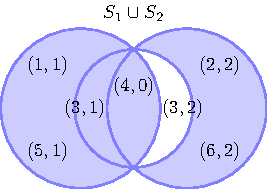
\includegraphics{fig_model_venn.pdf}
  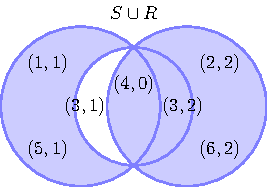
\includegraphics{fig_model_venn_reverse.pdf}
  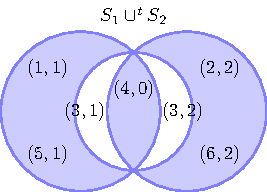
\includegraphics{fig_model_venn2.pdf}
  \caption{Venn diagrams for set and temporal set union operations of
    \acro{TSMS}}
  \label{fig:model:venn}
\end{figure}


\begin{example}\label{ex:model:s1s2}
  Let $R=\{(1,1), (3,1), (4,0), (5,1)\}$ and $S=\{(2,2), (3,2), (4,0),
  (6,2)\}$ be two time series. The union of $R$ and $S$ is $R\cup
  S=\{(1,1), (2,2), (3,1), (4,0), (5,1), (6,2)\}$. Because union is
  not symmetric, $S\cup R=\{(1,1), (2,2), \allowbreak(3,2), (4, 0), (5,1),
  (6,2)\}$. The temporal union results in $R\cupt S= S \cupt
  R=\{(1,1), (2,2), (4,0), (5,1), (6,2)\}$.  
  %
  Venn diagrams for all three cases are shown in
  Figure~\ref{fig:model:venn}, where the coloured area depicts the
  result time series. In every diagram, the central intersection area
  contains measures that share both time and value attributes, like
  instance $(4,0)$. The central left area contains the measures in $R$
  that only share the time attribute with a measure in $S$, like
  instance $(3,1)$. The central right area has a symmetrical
  meaning. The left and right outer areas are the remaining measures
  of $R$ and $S$ respectively.
\end{example}




Time series \emph{difference} can also be defined. Like union, the
difference requires both time series to have the same domain.
%
Let $R$ and $S$ be two time series and let $\dom R = \dom S$.
%
The \emph{difference} between $R$ and $S$, written $R-S$, is a time
series $R-S=\{m|m\in R\wedge m\notin S\}$.
%
The \emph{temporal difference} between $R$ and $S$, denoted $R-^t S$, 
is a time series $R-^t S=\{m|m\in R\wedge m \notinst S\}$.


Based on union and difference we can define \emph{intersection} as
$R\cap S = R - (R - S)$ and \emph{symmetric difference}
as $R \ominus S = (R - S) \cup (S - R)$. The
corresponding temporal operations can also be defined.


Relational \acro{DBMS} extend the set operators by some more such as
selection, rename or join. This kind of operators also make sense for
time series. To illustrate this possibility we define the join
operator.

Roughly speaking, the join of two time series is the combination of
measures sharing the same time attribute.  Let $R$ and $S$ be two time
series.  The \emph{join} of $R$ and $S$, denoted $R \join S$, is a
multivalued time series $R \join S = \{ (t,v_1,v_2) | (t,v_1) \in
R\wedge (t,v_2) \in S\}$. Note that $\dom(R\join
S)=\dom R\times\dom S$.
%
It must be noted that join requires both time series measures to share
exactly the same times. When time series diverge, the temporal
function operations explained later can be applied to adjust the time
instants to join requirements.


A \acro{DBMS} requires computational operators to provide opportunity
to calculate using the data contained. Relational \acro{DBMS} supply
operators like extend, aggregate or
summarise~\cite{date:introduction}. For time series, we define the more
general computational operators \emph{map} and \emph{fold}.

The map operator transforms a time series $S$ into a new time series
$R$ by applying a function to every measure.  Let $S$ and $R$ be two
time series, let $\cal{V}=\dom S$ and $\cal{V'}=\dom R$, and let
$f:\cal{T}\times\cal{V}\rightarrow\cal{T}\times\cal{V'}$ be a function
over a measure returning a measure. The \emph{map} of $f$ over $S$ is
a new time series defined as $\map(S,f)=\{f(m)|m\in S\}$. Note that
$\dom(\map(S,f))=\cal{V'}$.
%


The fold operator recursively combines every measure of a time
series. Assuming that $\mathcal{P}(C)$ is the powerset of $C$, we
define fold as follows.
%
Let $S=\{m_0,\dots, m_k\}$ and $R$ be two time series, let
$\mathcal{V}=\dom S$, let $\mathcal{V'}=\dom R$ and let 
%
$f:\mathcal{P}(\mathcal{T}\times\mathcal{V'}) \times (\mathcal{T}\times\mathcal{V}) \rightarrow \mathcal{P}(\mathcal{T}\times\mathcal{V'})$ 
%
be a function over a time series and a measure, which returns a time
series.
%
The \emph{fold} of $S$ by $f$ with initial value $R$ is a new time
series defined as $\fold(S,R,f) = f(\cdots(f(f(f(R,m_0),\allowbreak
m_1),\allowbreak m_2)\cdots),\allowbreak m_k)$.
%



The classical aggregation operator combines the data of a time series
into a single value.  It is worth to note that it is a special
case of fold.

Let $S=\{m_0,\dots,m_k\}$ be a time series, let $\mathcal{V}=\dom S$,
let $m$ be a measure with $\dom m=\mathcal{V}$, and let 
%
$f:(\mathcal{T}\times\mathcal{V})\times(\mathcal{T}\times\mathcal{V})\rightarrow \mathcal{T}\times\mathcal{V}$ 
%
be a function over two measures returning a measure. The
\emph{aggregate} of $S$ by $f$ with initial value $m$ is a new time
series defined as $\agg(S,m,f) = f(\cdots(f(f(f(m,m_0),\allowbreak
m_1),\allowbreak m_2)\cdots),\allowbreak m_k)$.  

% In the previous fold, the measures are computed in random order.
% However in some computational operations it is necessary to define the
% order, especially when $f$ is not commutative.  Then, it is possible
% to define a \emph{fold with order} as an extension of fold where
% measures are computed in a predetermined order.

% We define a
% \emph{fold with order}, $\orderfold$, as an extension of fold with a
% function $o$ that selects measures in order where $o: S_a \mapsto m_r$
% \[
%  \orderfold(S,S_i,f^f,o) =
%   \begin{cases}
%     S_i  \text{ if } |S|=0, \\
%     \orderfold(S_o,f^f(S_i,m_o),f^f,o)  \text{ else}
%   \end{cases}
% \]
% where $m_o = o(S)$ and $S_o = S - \{m_o\}$.



\begin{example}
\label{ex:computational-operators}
Let $S=\{(1,1),(2,3),(4,1)\}$ be a time series.  Map operator allows
computing a new time series whose values result from time multiplied
by value.  We define the map function $f(t,v)=(t,t\cdot v)$. Then
$\map(S,f)=\{(1,1),(2,6),(4,4)\}$.  
%


The aggregate operator allows, for instance, to compute the measure
that results from the sum of all the values.  To illustrate it, we
define the aggregate function $f(m,n)=(0,V(m)+V(n))$. Now,
$\agg(S,(0,0),f) = (0,5)$, where $5$ is the sum of all the values of
$S$. Note that time is meaningless in this computation.

The fold operator allows, for instance, to select the measures having
its value equal to one.  We define the fold function $f(R,m)=R\cup R'$
where $R'=\{m\}$ if $V(m)=1$ or $R'=\emptyset$ otherwise. Let $m$ be
any measure, note that $f(\emptyset,m)= R'$. Then
$\fold(S,\emptyset,f)=\{(1,1),(4,1)\}$.
\end{example}

%%%%%%% BINARY COMPUTATIONAL OPERATORS

Finally we describe how, using the operators defined before, we can
implement \emph{binary computational} operators between two time
series. This illustrates the power of the operators defined so far.
%

The strategy requires first to join the two time series and then
apply the computational operations. 
%
Let $S$ and $R$ be two time series and $\odot$ be a binary operator on
the value domain. The operator $\odot$ can be extended to the time
series as:
%
$S\odot R=\map(S\join R, f)$ being $f$ the function
$f(t,v,w)=(t,v\odot w)$.
%
This allows to extend real binary operations such as sum, $R+S$, or
division, $R/S$, to time series.


\subsubsection{Sequence operations}
\label{sec:sequence}

Sequence operations manipulate time series considering measures as
being totally ordered by time.  We define three basic operations:
\emph{slice}, \emph{successor} and \emph{concatenation}.


The classical interval concept can be applied to time domain. In this
context, given two time instants $s$ and $t$, we use the notation
$[s:t]$, $(s:t)$, $[s:t)$ and $(s:t]$ respectively for the closed
interval, open interval, open right and open left interval.
%
Following~\cite{last:hetland}, to slice a time series $S$ means to
extract a new time series $R\subseteq S$ constrained to a given time
interval. We denote this operation as the original time series followed
by the interval. Therefore, $S[s:t]=\{m|m\in S \wedge
T(m)\in[s:t]\}$. We can use other intervals to slice a time series in
a same fashion. For instance, $S(s:t]=\{m|m\in S \wedge
T(m)\in(s:t]\}$.

The ordinary time order allows to define the concepts of successor and
predecessor for the measures of a time series.
%
Let $S=\{m_0,\ldots,m_k\}$ be a time series and $m$ be an arbitrary
measure.
%
We say that $m_i=\nex_S(m)$ is the \emph{next} measure to $m$ in $S$ if and
only if $m_i=\inf(S(T(m):+\infty])$.  
%
We also say that $m_i=\prev_S(m)$ is the \emph{previous} measure to
$m$ in $S$ if and only if $m_i=\sup(S[-\infty:T(m)))$. 
%
Infinite measures are obtained when next and previous are applied to
supremum and infimum measures respectively: $\nex_S(\sup
S)=(+\infty,\infty)$ and $\prev_S(\inf S)=(-\infty,\infty)$.

To concatenate two time series means to compute a new time series with
the measures of the first time series followed in time order by the
measures of the second one. 
%
The concatenation requires both time series to share the same domain.
Let $R$ and $S$ be two time series and let $\dom R=\dom S$. The
\emph{concatenation} of $R$ and $S$, denoted as $R||S$, is a time
series that contains all the measures of $R$ together with those of
$S$ that do not intersect with the time interval of $R$. That is,
$R||S= R\cup (S - S[T(\inf R):T(\sup R)])$.



\subsubsection{Temporal function operations}
\label{sec:model:tfunc}

A time series can be thought as discrete representation of an
(original) temporal function. In this section we devise some
operations that manage the time series according to this temporal
function standpoint.  
%

The graph of a function allows to obtain and interpret the
continuous nature of a time series, when the domain of time and value
attributes can be plotted then the graph is equivalent to a graphical
representation.  
%
Let $S$ be a time series and $\cal{T}$ the time domain. The \emph{graph} of
the time series $S$ is a set of ordered pairs $\graph S
=\{(t,S(t))|t\in \cal{T}\}$ where $S(t)$ is a \emph{temporal representation
function} for the time series.
%


Given a time series $S$, the \emph{temporal representation function}
$S(t)$ is a function along the variable $t$ in the domain of
time and the target in the domain of values.
%
In some sense, $S(t)$ can be thought as the original temporal function
from which $S$ was obtained.
%

There is not an unique way to obtain $S(t)$ for a given time series
$S$. Because of this, in temporal representation functions we will
introduce a superscript, say $r$, that shows the name $r$ of the
representation method used. Then, $S(t)^r$ means the representation
function of $S$ using method $r$. Below, we exemplify the
representation functions using two different methods based on impulse
and constant piecewise functions.


\begin{definition}[Dirac representation] 
  Dirac delta (\dd) is a method of representation based on the Dirac
  delta function. Let $S$ be a time series. We define $S(t)^\dd$ as
  the following \dd{} representation function:
  \[
  S(t)^\dd
  =  \begin{cases}
          V(m) & \text{if } \exists m\in S:t=T(m) \\
          0    & \text{otherwise}
  \end{cases}
  \]
\end{definition}

\begin{definition}[Zohe representation]
  Zero-order hold everted (\zohe{}) is a method of representation
  based on the \emph{zero-order hold} signal reconstruction method. It
  is a piecewise constant function built from left-continuous step
  functions.  Let $S$ be a time series. We define $S(t)^\zohe$ as the
  following representation function:
  \[
  S(t)^\zohe 
  = \begin{cases}
    V(m) & \text{if } \exists m\in S: t\in \big(T(\prev_S(m)):T(m)\big]\\
    0    & \text{if } t > T(\max(S)) 
  \end{cases}
  \]
\end{definition}




The concept of representation is used for formalising some set and
sequence operators as temporal operators. 

% Consequently, the result of each one will depend on a representation
% method, which is indicated as a parameter.


We define a temporal interval operation to introduce this concept.
Let $S$ be a time series, let $[s:t]$ be an interval of two time
instants and let $r$ be a representation method. The \emph{temporal
  interval}, denoted as $S[s:t]^r$, returns a new time series with
measures in the interval temporal range. That is, $S[s:t]^r = S(u)^r$
for all $u \in [s:t]$. This is a general definition difficult to
implement, so for every representation a particular temporal interval
must be interpreted:

\begin{itemize}
\item Let $S(t)^\dd$ be the \dd{} representation for $S$. The
  \emph{\dd{} temporal interval} is $S[s:t]^\dd = S[s:t]
  \cup \{m\} \cup \{n\}$ where $m=(s,0)$ and $n=(t,0)$.

\item Let $S(t)^\zohe{}$ be the \zohe{} representation for $S$. The
  \emph{\zohe{} temporal interval} is $S[s:t]^\zohe{} = S(s:t]
  \cup \{m\}$ where $m=(t,v)$ and $v= V(\inf( S[t:+\infty] ))$.
\end{itemize}



From temporal interval other operators can be defined such as temporal
selection, temporal concatenation, or temporal join. As example the
definition of temporal interval operation is given.


The temporal selection over a time series allows to change the
resolution in the context of a representation function.  Let $S$ be a
time series, let $T=\{t_0,t_1,\dotsc,t_k\}$ be a set of time instants, and let 
$r$ be a representation method. The \emph{temporal selection}, denoted as
$S[T]^r$, is a time series with measures in $T$ times computed in
coherence with the representation method $r$. That is, $S[T]^r = S[t_0:t_0]^r
\cup S[t_1:t_1]^r \cup \dotsb \cup S[t_k:t_k]^r$. Let $t$ be a time
instant, note that temporal selection depends on the temporal interval
operation $S[t:t]^r$, which is equivalent to the notion of
temporal representation function over a single time instant. That is, $S[t:t]^r
= \{ (t, S(t)^r) \}$.




The temporal selection operation also allows to regularise a irregular
time series. Let $S$ be a time series, let $d,e\in\cal{T}$ be the
desired regularity parameters, and let $k\in\N$ be a limit for the
scope of the range.  A regularised $S$ can be obtained with $S[T]^r$
where $T = \{e+nd | n\in\N \wedge n\leq k \}$ is a set of time
instants equi-spaced.






\section{Multiresolution model}
\label{sec:MTSMS}

In this section we formalise a model for \acro{MTSMS}. Illustration
examples of the definitions given can be found at the end of the
section. Furthermore, in Section~\ref{sec:features} we have
intuitively introduced the concept of multiresolution through an
example.

A \acro{MTSMS} is a \acro{TSMS} that stores time series using a lossy
compression approach. 
%
The \acro{MTSMS} model is based on the concepts of \emph{measures} and
\emph{time series} as defined in Section~\ref{sec:model:TSMS}. We call
\emph{multiresolution time series} to each time series stored in a
\acro{MTSDB}.
%
A multiresolution time series is a collection of \emph{resolution
  subseries} that store a view of the original time series in a given
resolution.
%
The operator that adds data to a resolution subseries requires to
temporarily accumulate measures in a \emph{buffer}. This allow to
aggregate original data to obtain the expected resolution and finally
store them in a \emph{disc}.


\begin{figure}
  \centering
  %\begin{tikzpicture}
 \tikzset{
        myarrow/.style={->, >=latex',  thick},
      }
      

  \node[rectangle,draw,minimum height=6cm,minimum width=9cm] (m) {};
  \draw[shift=( m.south west)]   
  node[above right] {base de dades multiresolució};


  %discmig
  \node (m.center) (discr1) {...};

  %discr
  
  \node[ellipse,draw,minimum height=3.5cm,minimum width=2.5cm,alias=discr0] [left=of discr1] {};
  \node[above=0cm of discr0.north] {R0};
  \node[below=0cm of discr0] {disc resolució};

  \node[cylinder, draw, shape border rotate=90, aspect=0.25,alias=buffer0] [below=3mm of discr0.north] {buffer};
  \node[circle, draw,alias=disc0]  [above=3mm of discr0.south] {disc} ;
  \draw [->] (disc0.center)++(.4:.4cm) arc(0:180:.4cm);
  \draw[myarrow] (buffer0.bottom) -- (disc0.north);


  %discrd

  \node[ellipse,draw,minimum height=3.5cm,minimum width=2.5cm,alias=discrd] [right=of discr1] {};
  \node[above=0cm of discrd] {Rd};
  \node[below=0cm of discrd] {disc resolució};

  \node[cylinder, draw, shape border rotate=90, aspect=0.25,alias=bufferd] [below=3mm of discrd.north] {buffer};
  \node[circle, draw,alias=discd]  [above=3mm of discrd.south] {disc} ;
  \draw [->] (discd.center)++(.4:.4cm) arc(0:180:.4cm);
  \draw[myarrow] (bufferd.bottom) -- (discd.north);



  %mesura 
  \node[above=1cm of m.north] (m0) {};

  \draw[myarrow] (m0) -- (m.north) 
  node[right,midway] {mesura};

  \draw[myarrow] (m.north) -- (buffer0);
  \draw[myarrow] (m.north) -- (bufferd);
  \draw[myarrow] (m.north) -- (discr1);

\end{tikzpicture}
  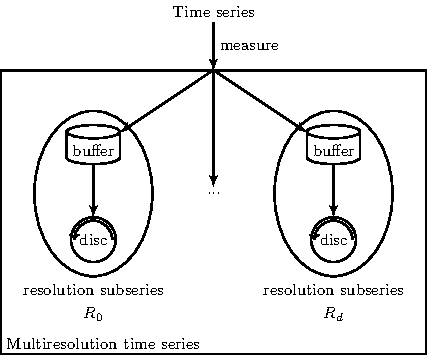
\includegraphics{fig_model_mtsdb.pdf}
  \caption{Architecture of \acro{MTSMS} model}
  \label{fig:model:mtsdb}
\end{figure}

Figure~\ref{fig:model:mtsdb} shows the architecture of a
\acro{MTSMS} for a single multiresolution time series.
%
In this way, the original time series gets stored in the resolution
subseries, each with a different time resolution and distinct
attribute aggregation policies. Discs are size bounded so they only
contain a fixed amount of measures. When a disc becomes full it
discards a measure. Thus, a multiresolution database is bounded in
size and the time series gets stored in a number of storage bounded
time subseries.

Regarding operations, the \acro{MTSMS} model requires two kind of
operators. Some operators should be devoted to set up the time
intervals between measures and to aggregate the attributes. Some other
operators should be dedicated to query the multiresolution schema and
to extract the time series data.

Following, we define the \acro{MTSMS} model structure and the
structural operators, the operations to query a multiresolution
schema, and the \emph{attribute aggregate functions}.  Although schema
manipulation operations could be defined, in this paper we exclusively
focus on structure and data query operators.


\subsection{Structure}

A \emph{buffer} is a container for a time series. The aim of the
buffer is to regularise the time series using a constant
\emph{resolution step} and an \emph{attribute aggregate function}.  We
name \emph{consolidation} to this action of regularisation.  Note that
the attribute aggregate functions are defined in
Section~\ref{sec:model:interpolador}.

\begin{definition}[Buffer]
  Let $S$ be a time series, let $\tau\in\cal{T}$ be the last
  consolidation time, let $\delta\in\cal{T}$ be the resolution step
  and let $f$ be an attribute aggregate function. We define a
  \emph{buffer} $B$ as the tuple $B=(S,\tau,\delta,f)$.
\end{definition}

An empty buffer is noted as $(\emptyset, t_0, \delta, f)$, that is an
empty time series, an initial consolidation time $t_0\in\cal{T}$, a
resolution step $\delta$ and a function $f$.  Given a buffer all the
consolidation time instants can be determined as $\tau_n=t_0+n\delta$
for all $n\in\N$.

Let $B=(S, \tau, \delta, f)$ be a buffer. The \emph{consolidation} of
$B$ is an operation that computes a new measure $m=f(S, \tau, \delta)$
summarising the data of $S$ comprised in the given interval.

A buffer has two main structural operations. The first one adds a
measure to the buffer and the second one consolidates the buffer.

Let $B=(S,\tau,\delta,f)$ be a buffer and let $m$ be a measure.  The
addition of $m$ to $B$, noted as $\addB(B,m)$, returns a new buffer
$\addB(B,m)=(S',\tau,\delta,f)$ where $S' = S \cup \{m\}$.

Let $B=(S,\tau,\delta,f)$ be a buffer. The consolidation of $B$, noted
as $\consB(B)$, returns a new buffer and a new measure $\consB(B)=(B',m')$
where $ B'= (S[\tau+\delta:+\infty], \tau+\delta,\delta,f)$ and $m' =
f(S,\tau,\delta)$. Note that after the consolidation, the
consolidated part of the time series can be removed from the buffer:
historic data is discarded.

The consolidation of a buffer is applied to the first non consolidated
time instant and the total consolidation is obtained by successive
application of the operator. 
%
This requires measures to be added by time order and to consolidate
the buffer when the time of some measure is bigger than the buffer's
next consolidation time.  
%
Let $B=(S,\tau,\delta,f)$ be a buffer and $m=\sup S$ the maximum
measure of $B$. We say that $B$ is consolidable if and only if $T(m)
\geq \tau+\delta$.

A \emph{disc} is a finite capacity container of measures. A time
series stored in a disc has its cardinal bounded. When the cardinal of
the time series is to overcome the limit, some measures need to be
discarded.

\begin{definition}[Disc]
  Let $k\in\N$ and $S$, $|S|\leq k$, be a time series. We define a
  \emph{disc} $D$ as the tuple $D=(S,k)$.
\end{definition}

An empty disc is noted as $(\emptyset,k)$. It is the tuple of an
empty time series and a bound $k$.

The main operation on a disc is to add a measure while keeping under
control the cardinal of the times series. Let $D=(S,k)$ be a disc and
let $m$ be a measure.  The addition of $m$ to $D$, written as
$\addD(D,m)$, is a new disc $\addD(D,m)=(S',k)$ where
%
\[
S' = \begin{cases}
  S\cup\{m\}                 & \text{if } |S|<k  \\
  (S-\{\min S\}) \cup \{m\} & \text{otherwise}
\end{cases}  
\]

A \emph{resolution subseries} is a structure that regularises and
aggregates a time series. It is composed of a buffer, which contains
the time series to be regularised, and a disc, which contains
the regularised time series.


\begin{definition}[Resolution subseries]
  Let $B$ be a buffer and let $D$ be a disc.  We define a
  \emph{resolution subseries} $R$ as the tuple $R=(B,D)$.  
\end{definition}
 
The operators of a resolution subseries extend the buffer and disc
ones. Let $R=(B,D)$ be a resolution subseries and let $m$ be new a
measure.  The addition of $m$ to $R$, noted as $\addR(R,m)$, is a new
resolution subseries $\addR(R,m)=(B',D)$ where $B'= \addB(B,m)$ is the
addition of the measure to the buffer.  The consolidation of $R$,
noted as $\consR(R)$, is a new resolution subseries
$\consR(R)=(B',D')$ where $(B',m') = \consB(B)$ is the consolidation
of the buffer and $D'= \addD(D,m')$ is the addition of the
consolidated measure to the disc. A resolution subseries is
consolidable only when its buffer is consolidable.

A \emph{multiresolution time series} is a set of resolution subseries
referred to the same time series. We store a time series regularised
with distinct resolutions across the resolution subseries, as
previously shown in Figure~\ref{fig:model:mtsdb}.

\begin{definition}[Multiresolution time series]
  Let $M=\{R_0, \dots, R_k\}$ be a finite set of resolution
  subseries. Then $M$ is a \emph{multiresolution time series}.
\end{definition}

Therefore, to define a multiresolution time series we must define the
number of resolution subseries and its corresponding parameters
$(\delta,\tau,f,k)$.  Usually there are no repeated pairs of
$(\delta,f)$ parameters among a multiresolution series, so they act as
key attributes.

The operators of a multiresolution time series apply to every
resolution subseries contained. Let $M=\{R_0,\allowbreak
\dots,\allowbreak R_k\}$ be a multiresolution time series and let $m$
be a measure.
%
The addition of a measure to every resolution subseries, noted as
$\addM(M,m)$, is a new multiresolution time series $\addM(M,m)=\{R'_0,
\dots,\allowbreak R'_k\}$ where $R'_i=\addR(R_i,m)$. The consolidation
of all resolution subseries, noted as $\consM(M)$ is a new
multiresolution time series $\consM(M)=\{R'_0,\allowbreak
\dots,\allowbreak R'_k\}$ where
\[R'_i=
\begin{cases}
\consR(R_i) & \text{if } R_i \text{ consolidable}\\
 R_i & \text{otherwise}
\end{cases}
\]

% The multiresolution consolidation operation should be applied
% regularly based on a consolidation clock. When the measure ordered
% addition approach is taken as explained in the buffer's consolidation,
% then there is no need for a clock in a \acro{MTSMS}. The consolidation
% clock is induced by the measure's addition and then it is only
% necessary to check the multiresolution consolidation operation on new
% additions. However, there could be other approaches where the
% consolidation clock was given by an external clock or external
% events. Then the consolidable definitions would depend on this
% external clock.





\subsection{Queries}

There are two basic time series queries for a \acro{MTSMS}: (i) to
extract a time subseries from a resolution subseries or (ii) to query
for a total time series from all consolidated data.

% Aquesta sembla una consulta una mica circumstancial i menor ...
Let $M$ be a multiresolution time series and let $(\delta,f)$ be a
pair of key attributes.  The first query, denoted as
$\seriedisc(M,\delta,f)$, is a time series such that $\exists (B,D)
\in M: B=(S,\tau,\delta,f) \wedge D=(\seriedisc(M,\delta,f), k) $
where $S,\tau,k$ are bound variables.  Note that we
assume there are no repeated $(\delta,f)$ pairs in $M$.

Let $M=\{R_0,\dots,R_k\}$ be a multiresolution time series and let
$S_0,\dots,S_k$ the time series corresponding to the resolution
subseries $R_0,\dots,R_k$. Assume that the attribute aggregation
functions of all $R_i$ are the same and the resolution steps of all
$R_i$ are distinct.
%
We note as $\totalseries(M)$, the time ordered concatenation of all
time subseries. Recall that $R||S$ is the concatenation for two time
series $R$ and $S$, which has been defined in
Section~\ref{sec:sequence}. Assume that $i_0,\dots,i_k$ is a
permutation of $[0,k]$ such that $\delta_{i_0} < \delta_{i_1} < \cdots
< \delta_{i_k}$ being $\delta_i$ the resolution step of the resolution
subseries $R_i$. Then, $\totalseries(M) = S_{i_0} || S_{i_1} || \cdots
|| S_{i_k}$.
%
TotalSeries obtains the better possible resolution.

From these aforementioned basic time series queries, more elaborated
queries can be applied to \acro{MTSMS} by using \acro{TSMS}
operations. For example, let $L$ and $M$ be two multiresolution time
series, we can compute the sum of both as $\totalseries(L) +
\totalseries(M)$. Recall that $R+S$ is the sum of the values of two
time series $R$ and $S$, which has been defined in
Section~\ref{sec:set} as a binary computational operator.


\subsection{Attribute aggregate function}
\label{sec:model:interpolador}

Attribute aggregate functions are a specific case of \acro{TSMS}
aggregate operations used to summarise time series data while
consolidating a buffer.
%
% Let $S$ be a time series and let $[x,v]$ be a
% time interval. An attribute aggregate function $f$ calculates a new
% measure $m=f(S,[x,v])$. Then, this resulting measure $m$ is interpreted to
% summarise the measures of $S$ for the consolidation interval $[x,v]$.

Let $S$ be a time series, let $\delta$ be a resolution step and let
$\tau$ be a consolidation time.  An \emph{attribute aggregate function} $f$
calculates a new measure $m=f(S,\tau,\delta)$. From $\tau$ and
$\delta$, we obtain the time interval $[\tau:\tau+\delta]$.  Then, the
resulting measure $m$ is interpreted to summarise the measures of $S$
for the time interval $[\tau:\tau+\delta]$.



% \[
% f : S=\{m_0,\ldots,m_k\} \times I=[t_i,t_j] \mapsto m'
% \]
% \[
% f: \cal{P}(\cal{T}\times\cal{V}) \times (\cal{T}\times\cal{T}) \rightarrow \cal{T}\times\cal{V}
% \]

An attribute aggregation function follows this general schema. First,
it obtains a time subseries $S'$ according to the consolidating
interval using a slice operator. For example, $S' =
S[\tau:\tau+\delta]$. Second, it applies a \acro{TSMS} aggregation
function on this time subseries to obtain $m$. For instance, $m =
\agg(S',n, f)$, being $f$ an aggregation function and $n$ an initial
measure, as defined in Section~\ref{sec:set}.

Many different attribute aggregate functions can be used in order to
summarise a time series, for example it is possible to calculate an
statistic indicator of the time series such as the average or a more
complex digital signal processing operation as proposed
by~\cite{zhang11}. Furthermore, the representation of a time series
and some of its pathologies can be considered during the aggregation
process.

Given the diversity of attribute aggregate functions, no global
assumptions can be made about them. Each user should decide which
combination of aggregation and representation fits better to the
measured phenomena.  Therefore, the \acro{MTSMS} model must have a
generic design that allows the users to define their own aggregate
functions.

In what follows we will give some examples of usual attribute
aggregation functions. These functions compute a new measure given a
set of known measures. Then, an attribute aggregation function should
compute a new \emph{time} and a new \emph{value} from the set known measures.
%
% For the rest of this Section we will write $m=f(S,[x,v])$ be the
% resulting measure of an attribute aggregation function $f$ applied to
% a time series $S$ for a time interval $[x,v]$.

% Sobre el calcul del nou temps

The attribute aggregation functions generally return measures that
match the buffer consolidating times. Assume, for instance, that $f$
is an attribute aggregation function and let $m=f(S,\tau,\delta)$.
Then, the time of $m$ is usually computed as $T(m)=\tau+\delta$.
%
However, in some cases it is preferred that $T(m)$ do not match the
buffer consolidating times.
%
For instance, the resulting measure can be aggregated from a time
subseries $S'$ using an open interval $S'=S(\tau:\tau+\delta)$, a
closed interval $S'=S[\tau:\tau+\delta]$, or other combinations like
$S'=S(\tau-d:\tau+\delta-d]$, where $d$ is a time duration that delays the
consolidation to $T(m)=\tau+\delta-d$.
%
This time offset can also be variable. For example, an aggregate
function that returns the first measure of the interval
$m=\min(S[\tau:\tau+\delta))$, then the resulting time fulfils that
$\tau\leq T(m) < \tau+\delta$.

% Sobre el calcul del nou valor
Assume that $f$ is an attribute aggregation function and let
$m=f(S,\tau,\delta)$.  An attribute aggregation function $f$ should
compute the value of $m$.
%
Next there are some examples that illustrate how to compute $V(m)$
based on the temporal function time series operators. 
That is, the time series aggregated is interpreted by the temporal
representation function $S(t)^r$ as has been described in
Section~\ref{sec:model:tfunc}. 
%
In these example functions we leave the time series representation $r$
uninstantiated.

\begin{itemize}
\item The \emph{maximum} computes $V(m)$ as $V(m) =
  \max\limits_{\forall t \in [\tau:\tau+\delta]} S(t)^r$. It
  summarises $S$ with the maximum of the measure values in the
  interval $[\tau:\tau+\delta]$.
\item The \emph{last} computes $V(m)$ as $V(m) = S(\tau+\delta)^r$. It
  summarises $S$ with the value at $\tau+\delta$ time instant.
\item The \emph{mean} computes $V(m)$ as $V(m) = \frac{1}{\delta}
  \int\limits_{\tau}^{\tau+\delta} S(t)^r dt$. It summarises $S$ with
  the mean of the function in the interval $[\tau:\tau+\delta]$.
\end{itemize}

The time series representation in previous examples can be
instantiated in several ways. In what follows we exemplify this
instantiating $r$ as \dd{} and \zohe{}.

Dirac delta attribute aggregation functions interpret the resulting
time as centered on the interval $T(m)=\frac{2\tau+\delta}{2}$. The
resulting value $V(m)$ depends on the attribute, let
$S'=S[\tau:\tau+\delta]^\dd$ be the selection of measures by Dirac
delta temporal interval. Then,
\begin{itemize}
\item The $maximum^\dd$ is such that $V(m) =
  \max\big(0,\max\limits_{\forall n \in S'} V(n)\big)$.
\item The $last^\dd$ is such that $V(m) = V(\max S')$.
\item The $mean^\dd$ is such that $V(m) = \frac{1}{\delta}
  \sum\limits_{\forall n \in S'} V(n)$. Note that for the Dirac
  delta function $\int\dd(t)dt=1$.
\end{itemize}

Note that $\sum\limits_{\forall n \in S'} V(n)$ is a sum of values
that could be implemented as $\agg(S',(0,0),f)$ where
$f(m,n)=(0,V(m)+V(n))$, as shown in
Example~\ref{ex:computational-operators}.

\zohe{} attribute aggregation functions interpret the resulting time
as the right limit of the interval $T(m)=\tau+\delta$. The resulting
value $V(m)$ depends on the attribute, let
$S'=S[\tau:\tau+\delta]^\zohe{}$ be the selection of measures by
\zohe{} temporal interval. Then,

\begin{itemize}
\item The $\maxz$ is such that $V(m) = \max\limits_{\forall n \in S'}
  V(n)$.
\item The $last^\zohe{}$ is such that $V(m) = V(\max S')$.
\item The $\meanz$ is such that $V(m) = \frac{1}{\delta}
  \big[(T(o)-\tau)V(o) + \sum\limits_{\forall n\in R}( T(n)-
  T(\prev_S n) )V(n)\big]$ where $o=\min S'$ and $R= S' - \{o\}$.
\end{itemize}

Note that  $\meanz$ is a sum of values
that could be implemented as $\meanz = \frac{1}{\delta}\agg(S',(0,0),f)$ where $f(m,n)=(0,V(m)+v)$ and 
\[
 v= 
 \begin{cases}
   (T(n)-\tau)V(n) & \text{if } n=\min S'\\
   (T(n)-T(\prev_{S'} n))V(n) & \text{else }
 \end{cases}
\]

\emph{RRDtool}, \cite{rrdtool}, uses an aggregation function similar
to $\meanz$ to summarise velocity counter data by keeping the area
below the original signal.

It is interesting to note that some attribute aggregation patterns are
very similar. For instance, the maximum and last attribute aggregation
schemes differ basically on the interval selection operation. However,
other patterns have a more elaborated interpretation depending on the
actual representation used. This is the case of $\meanz$ and $mean^\dd$.


\begin{example}\label{ex:model:smultiresolution} 
  We define a multiresolution schema for a time series, we consolidate
  the database and we query its data.  Let $S = \{
  (1,6),(5,2),\allowbreak (8,5),\allowbreak (10,0),\allowbreak
  (14,1),\allowbreak (19,6),\allowbreak (22,11),\allowbreak
  (26,6),(29,0) \}$ be a time series and let $M=\{R_0,R_1\}$ be a
  multiresolution time series where each resolution parameters are
  $\tau_0=0$ , $\delta_0=5$, $f_0 =\meanz$, $k_0=4$ and $\tau_1=0$,
  $\delta_1=10$, $f_1 =\maxz$, $k_1=2$. Therefore $R_0$ will be
  consolidated at time instants 5, 10, 15, 20, 25, 30\dots and $R_1$
  at 10, 20, 30\dots

  All measures of $S$ are added to $M$
  and then it is consolidated until it is no more consolidable. As
  $T(\max S)=29$, the last consolidation times are $\tau_0=25$ and
  $\tau_1=20$, so we call $M_{29}$ to the multiresolution time series
  at this state.

  Then, the two time subseries consolidated are obtained by querying
  $\seriedisc(M_{29},5,\allowbreak \meanz)=\{\allowbreak
  (10,3),\allowbreak (15,\allowbreak 2),\allowbreak (20,7),\allowbreak
  (25,8)\}$ and $\seriedisc(M_{29},\allowbreak 10,\allowbreak \maxz)
  =\allowbreak \{ \allowbreak (10,6),\allowbreak (20,11)\}$. Regarding
  buffers, let $S_0$ and $S_1$ be the $M_{29}$ buffer's time series,
  note that $S_0= \{\allowbreak (26,6),\allowbreak (29,0)\allowbreak
  \}$ and $S_1=\{\allowbreak (22,11),\allowbreak (26,6),(29,0)\}$.

  In this particular example,
  $ \totalseries(M_{29}) = \seriedisc(M_{29},\allowbreak 5,\meanz)$ as $R_0$ has
  twice the resolution than $R_1$ and $k_0$ is bigger than $k_1$. 
\end{example}



%%% Local Variables:
%%% TeX-master: "main"
%%% ispell-local-dictionary: "british"
%%% End:

% LocalWords:  genericity multiresolution subseries consolidable

% LocalWords:  pathologies MTSMS TSMS cardinality multivalued infimum
% LocalWords:  multivalues supremum tuple affinely projectively MTSDB
%  LocalWords:  semitemporal piecewise TotalSeries RRDtool



%------- Annexos ------
\appendix

%------- Glossari ------
\cleardoublepage
%\phantomsection\addcontentsline{toc}{chapter}{\glossaryname}
%\pdfbookmark{\glossaryname}{bookmark:glossari}
\chapter{Nomenclatura i abreviacions}
\glsaddall
\printglossary
\printglossary[type=\acronymtype]
\printglossary[type=notation,nonumberlist,style=estil-notation]
%------- Bibliografia ------
\cleardoublepage
%\phantomsection\addcontentsline{toc}{chapter}{\bibname}
\pdfbookmark{\bibname}{bookmark:bibliografia}
\printbibliography
%----------------------------------------------

%\backmatter

\end{document}



%%%%%%%%%%%%%%%%%%%%%%%%%%%%%%%%%%%%%%%%%%%%%%%%%%%%%%%%%%%%%%%%%%%%%%%%%%  
% Model dels sistemes de gestió de bases de dades per sèries temporals.
%
% Copyright (C) 2011-2012 Aleix Llusà Serra.
% 
% This LaTeX document is free software: you can redistribute it and/or
% modify it under the terms of the GNU General Public License as
% published by the Free Software Foundation, either version 3 of the
% License, or (at your option) any later version.
%
% This document is distributed in the hope that it will be useful, but
% WITHOUT ANY WARRANTY; without even the implied warranty of
% MERCHANTABILITY or FITNESS FOR A PARTICULAR PURPOSE. See the GNU
% General Public License for more details.
%
% You should have received a copy of the GNU General Public License
% along with this document. If not, see <http://www.gnu.org/licenses/>.
%
%
% Aleix Llusà Serra
% Departament de Disseny i Programació de Sistemes Electrònics de la Universitat Politècnica de Catalunya (DiPSE-UPC)
% Escola Politècnica Superior d'Enginyeria de Manresa (EPSEM)
% Av. de les Bases de Manresa, 61-73
% 08242 Manresa (Barcelona)
% PAÏSOS CATALANS 
%
% aleix (a) dipse.upc.edu
% 
% El codi font LaTeX del document es troba a 
% <http://escriny.epsem.upc.edu/projects/rrb/>
%%%%%%%%%%%%%%%%%%%%%%%%%%%%%%%%%%%%%%%%%%%%%%%%%%%%%%%%%%%%%%%%%%%%%%%%%% 